\documentclass[aspectratio=169]{beamer}
\usetheme[style=noir]{fhtw}
\usepackage{preamble}
\resetcounteronoverlays{listing}

\title[Microcontroller]{Microcontroller}
\subtitle{\glsentrytext{ci} - ASSIST \glsentrytext{heidi}}
\author{Alija Sabic, \glsentrytext{msc}}
\mail{sabic@technikum-wien.at}
\institute{Department Electronic Engineering}

\begin{document}

\begin{frame}[plain]
    \titlepage
\end{frame}

\section{\glsentrydesc{uc}}

\subsection{Introduction}

\begin{frame}{What is a Microcontroller?}
    \par Microcontroller is a computer system in a single chip.
    \par Just like a \acs{pc}, it consists of:
    \begin{itemize}
        \item \acs{cpu} --- less powerful than a full blown desktop processor
        \item Persistent and non-persistent memory (\acs{hdd}, \acs{ram}) --- typically a few \SI{100}{\kibi\byte} of \acs{ram} instead of > \SI{1}{\gibi\byte} like a typical computer
        \item System clock --- not as fast as desktop processors, but many \acsp{uc} can also be clocked externally
        \item Peripherals --- provide interfaces found in the field of embedded systems (\acs{gpio}, \acs{i2c}, \acs{spi}, \acs{uart}, \acs{can}, \ldots) rather than interfaces found in desktop computers (\acs{pci}, \acs{pcie}, Thunderbolt \texttrademark, \acs{sata}, \ldots)
    \end{itemize}
\end{frame}

\begin{frame}{What is a Microcontroller?}
    \begin{figure}
        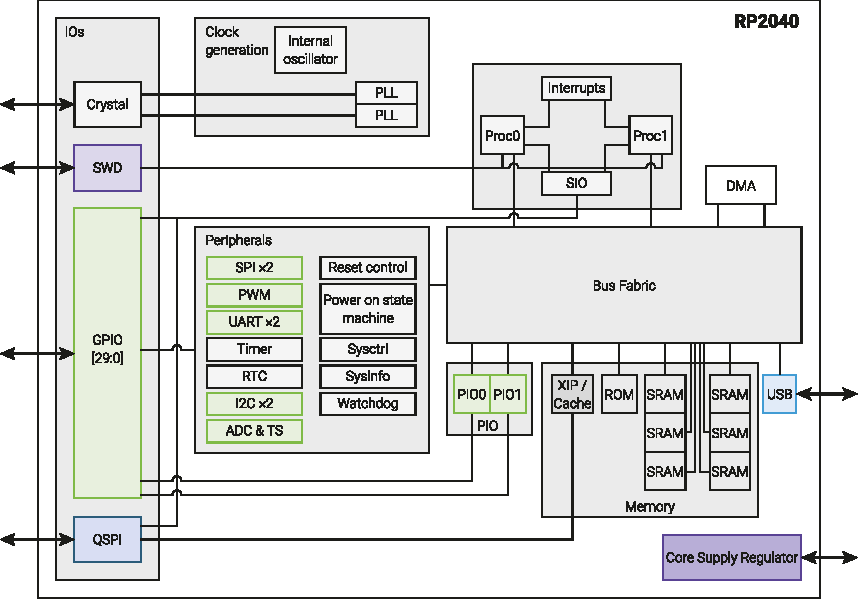
\includegraphics[width=0.9\textwidth]{microcontroller/arduino/rp2040/block-diagram.pdf}
        \caption{System overview of the RP2040 Chip}
    \end{figure}
\end{frame}

\begin{frame}{What is a Microcontroller?}
    \begin{figure}
        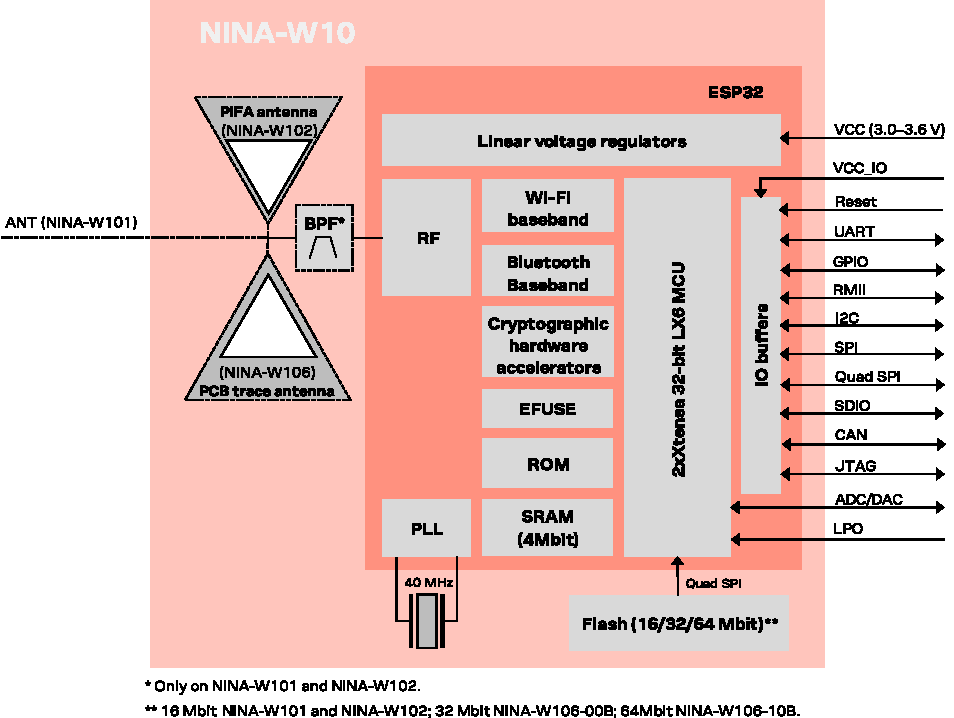
\includegraphics[width=0.9\textwidth]{microcontroller/nina-w10-block-diagram.pdf}
        \caption{Nina W10 Block Diagram}
    \end{figure}
\end{frame}

\begin{frame}{What is a Microcontroller?}
    \begin{figure}
        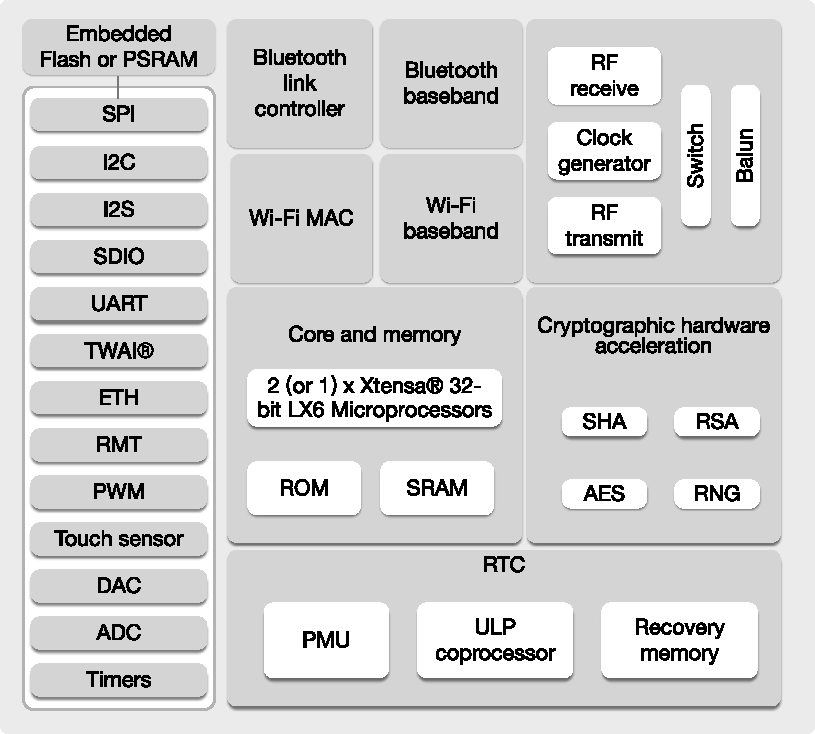
\includegraphics[width=0.7\textwidth]{microcontroller/esp32-functional-block-diagram.pdf}
        \caption{ESP32 Functional Block Diagram}
    \end{figure}
\end{frame}

\subsection{Examples}
\begin{frame}
    \begin{itemize}
        \item Pace makers and \ac{fes}
        \item Current pace makers have \SIrange{5}{7}{yrs.} battery life time
        \item Feedback loops $\rightarrow$ adapt to physical needs
        \item Multi-channel stimulation and measurment electrodes
    \end{itemize}
\end{frame}

\begin{frame}
\end{frame}

\begin{frame}
    \begin{itemize}
        \item Alternative computer input devices
        \item Implants and \acs{fes} devices
        \item Active prosthesis, orthesis and artificial limbs
        \item Environmental control systems
        \item Braille displays
    \end{itemize}
\end{frame}

\section{\glsentrydesc{es}s}

\subsection{Definition}

\begin{frame}
    \begin{definition}
        An embedded system is a computer system --- a combination of computer processor, computer memory, and input/output peripheral devices --- that has a dedicated function within a larger mechanical or electronic system (Source: \href{https://en.wikipedia.org/wiki/Embedded_system}{Wikipedia - Embedded Systems}).
    \end{definition}
    \vspace{-1em}
    \begin{figure}
        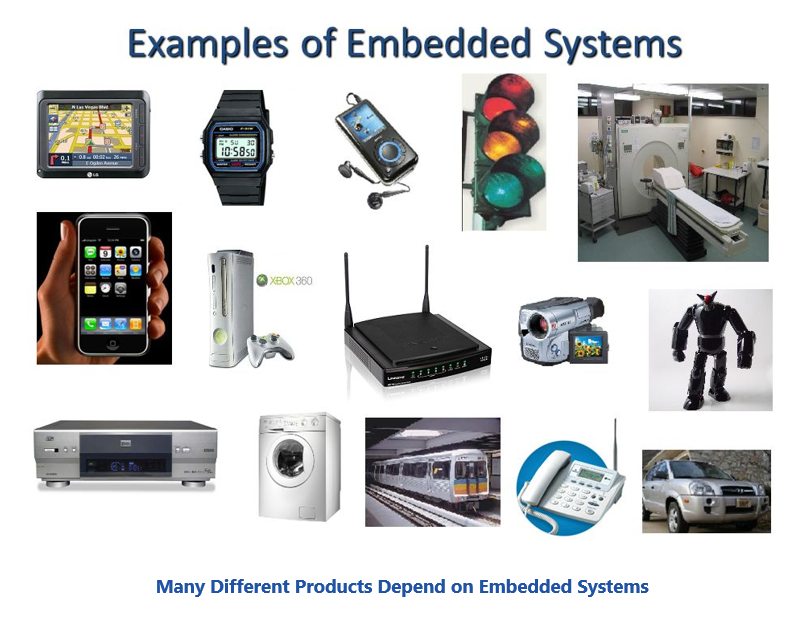
\includegraphics[width=0.5\textwidth]{microcontroller/embedded-system-examples.png}
        \caption{\glsentrydesc{es} examples.}
    \end{figure}
\end{frame}


\subsection{\glsentrydesc{os}}

\begin{frame}
    \resizebox{\linewidth}{!}{
        \begin{minipage}[t]{1.1\textwidth}
            \begin{itemize}
                \item<1-> Bare-metal programming
                    \begin{itemize}
                        \item ``Infinite loop''
                        \item Little or no software overhead
                        \item High control of hardware
                        \item Single-purpose or simple applications, hardware-dependent
                        \item Strict timing (e.g. motor control)
                    \end{itemize}
                \item<2-> \ac{rtos}
                    \begin{itemize}
                        \item Scheduler overhead
                        \item More powerful microcontroller required
                        \item High control of hardware
                        \item Multithreading, some common libraries
                        \item Multiple tasks: networking, user interface, etc.
                    \end{itemize}
                \item<3-> Embedded \ac{gpos}
                    \begin{itemize}
                        \item Large overhead (scheduler, memory management, background tasks, \ldots)
                        \item Microprocessor usually required (and often external \acs{ram} and \acs{nvm})
                        \item Low direct control of hardware (files or abstraction layers)
                        \item Multiple threads and processes, many common libraries
                        \item Multiple complex tasks: networking, file system, graphical interface, \ldots
                    \end{itemize}
            \end{itemize}
        \end{minipage}%
        \begin{minipage}[t]{0.35\textwidth}
            \onslide<1->{
                \begin{figure}
                    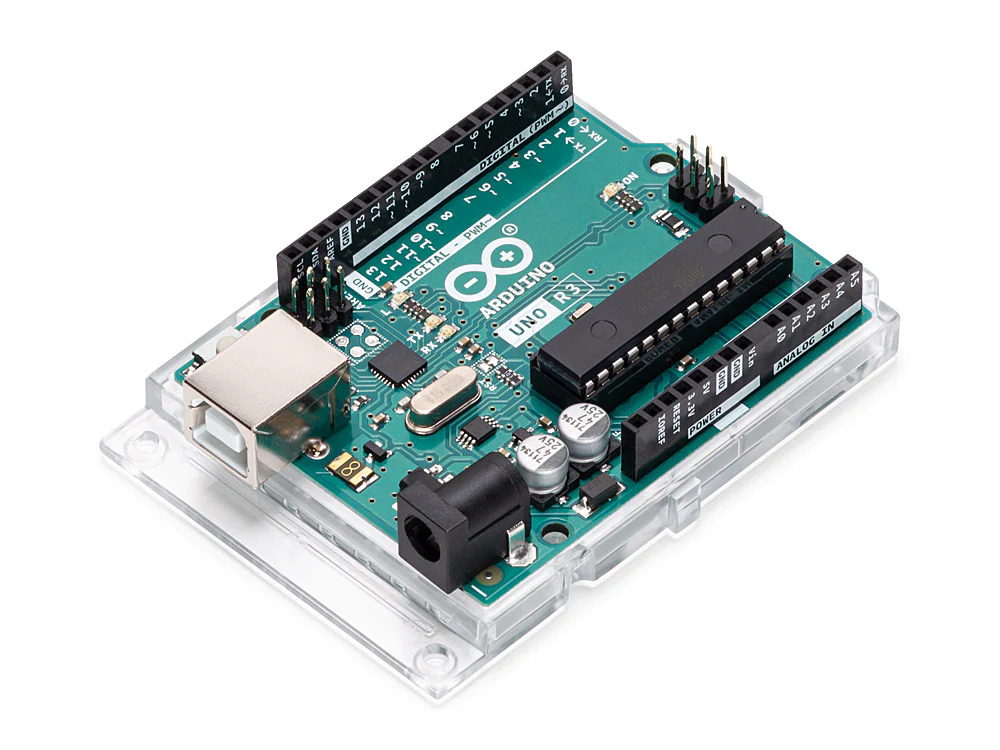
\includegraphics[height=2cm]{microcontroller/arduino/boards/uno.jpg}
                    \caption{\href{https://store.arduino.cc/products/arduino-uno-rev3}{Arduino\textregistered{} Uno}}
                \end{figure}
            }
            \onslide<2->{
                \begin{figure}
                    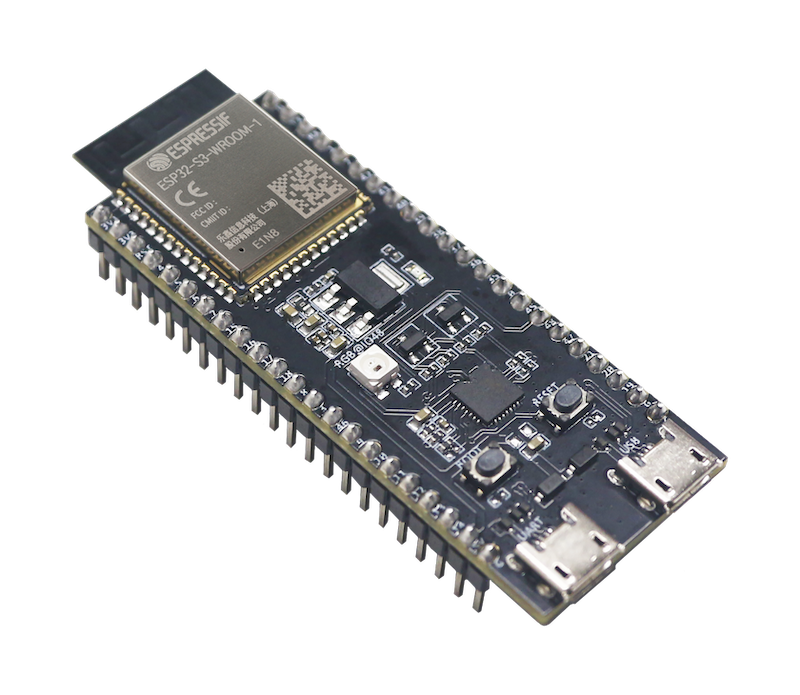
\includegraphics[height=2cm]{microcontroller/boards/esp32-s3-devkitc-1-v1-isometric.png}
                    \caption{\href{https://docs.espressif.com/projects/esp-idf/en/latest/esp32s3/hw-reference/esp32s3/user-guide-devkitc-1.html}{ESP32-S3 DevKitC-1}}
                \end{figure}
            }
            \onslide<3->{
                \begin{figure}
                    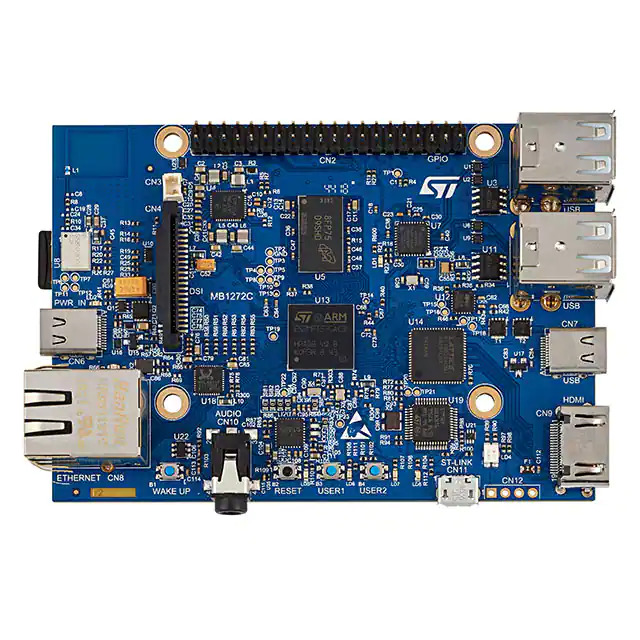
\includegraphics[height=2cm]{microcontroller/boards/stm32mp157d-dk1.jpg}
                    \caption{\href{https://www.st.com/en/evaluation-tools/stm32mp157d-dk1.html}{STM32MP157D-DK1}}
                \end{figure}
            }
        \end{minipage}
    }
\end{frame}

\begin{frame}
    \begin{figure}
        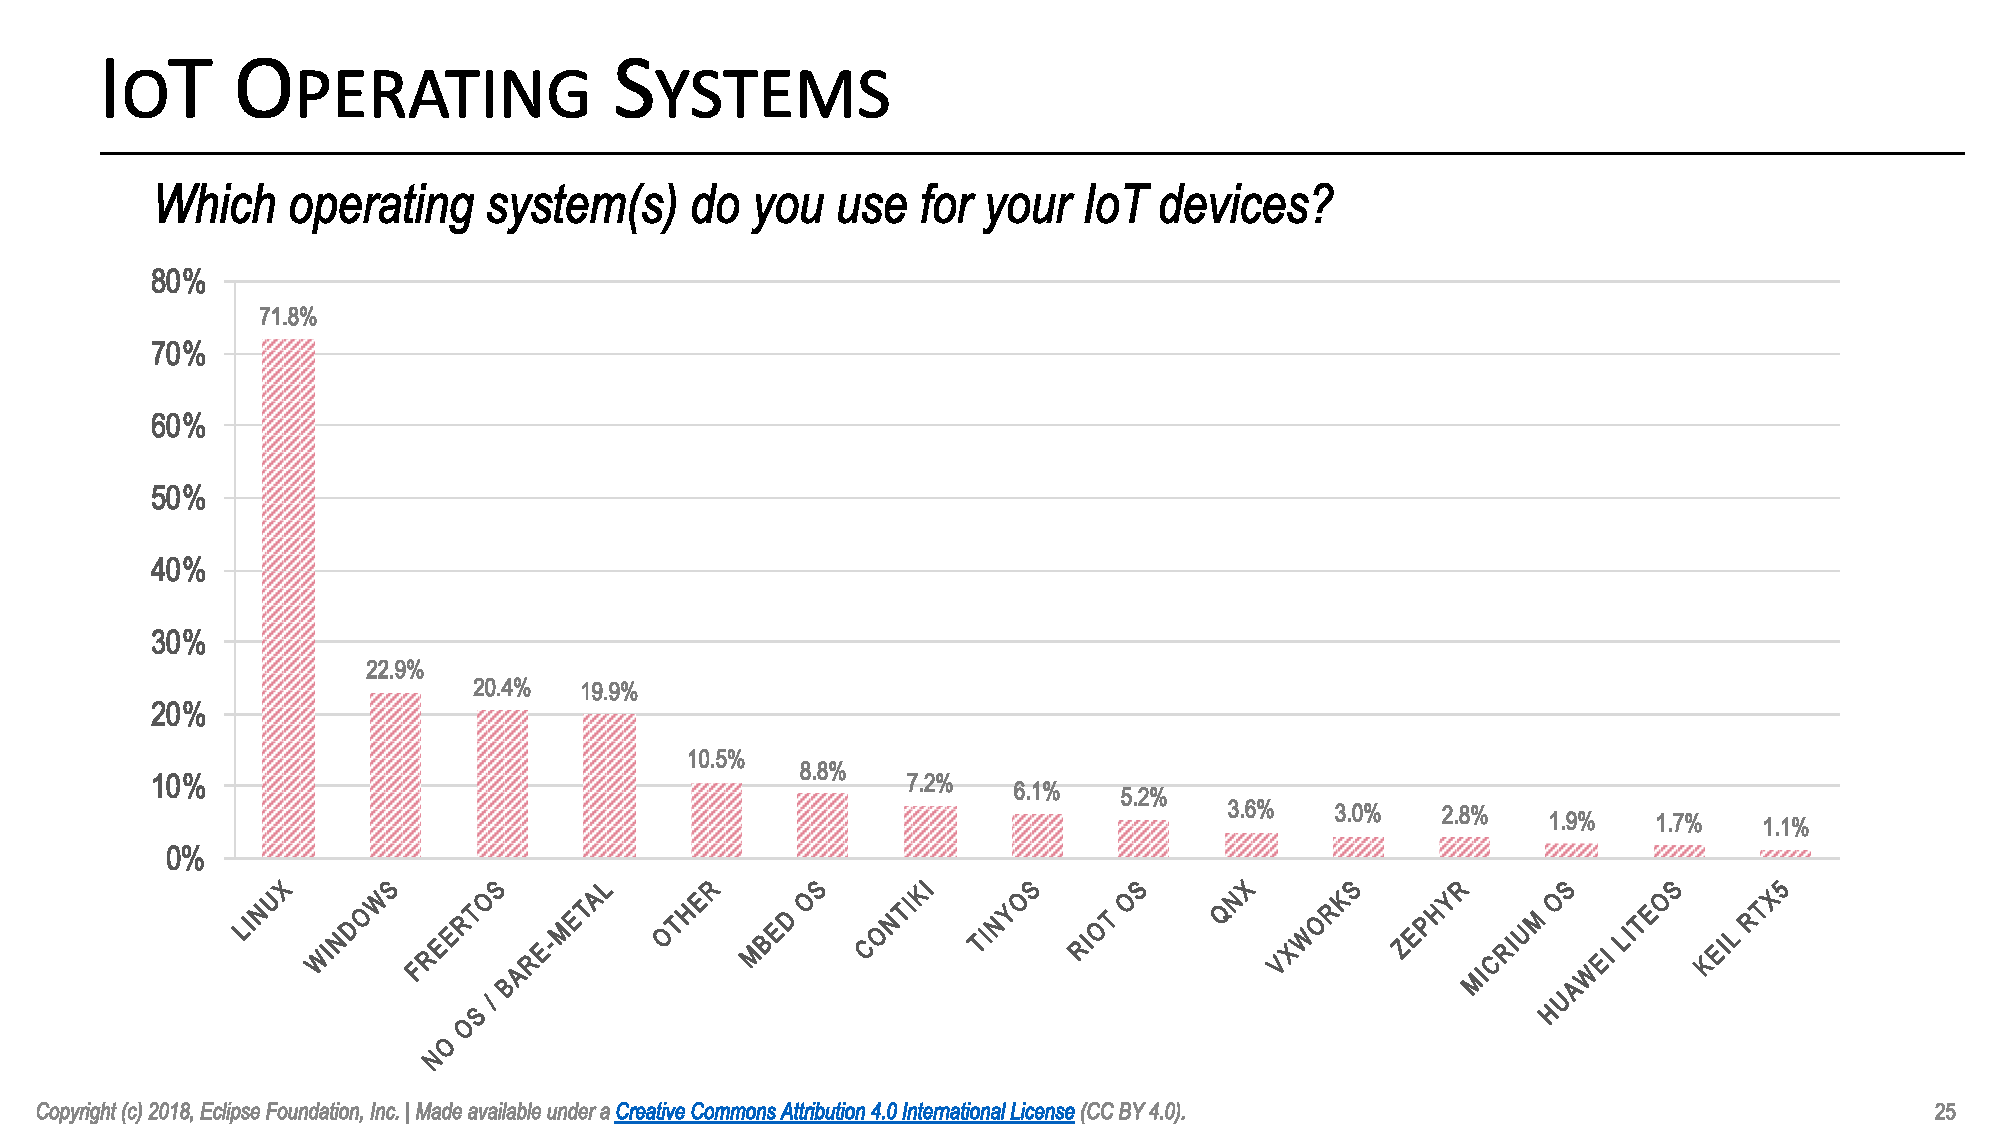
\includegraphics[width=\textwidth]{microcontroller/iot-developer-survey-2018-os.pdf}
        \caption{\href{https://iot.eclipse.org/community/resources/iot-surveys/assets/iot-developer-survey-2018.pdf}{Eclipse \glsentrytext{iot} Developer Survey}: \glsentrydesc{os}s}
    \end{figure}
\end{frame}

\section{Arduino\textregistered{}}

\subsection{What is Arduino?}

\begin{frame}
    % \begin{itemize}
    %     \item Arduino\textregistered{} is an \ac{ide} for microcontrollers, supporting many different application boards
    %     \item The software support makes it easy to use various hardware modules (e.g. \acsp{lcd}, servo motors, \ldots)
    % \end{itemize}
    \begin{itemize}
        \item Open-source electronics platform
        \item Designed for interactive projects and prototyping
        \item Easy-to-use hardware and software
        \item Popular among hobbyists, educators, and professionals
    \end{itemize}
    \par The Arduino\textregistered{} ``ecosystem'' consists of several integral compontents:
    \begin{itemize}
        \item Microcontroller boards (Arduino\textregistered{} boards)
        \item \ac{io} pins for connecting electronic components
        \item Arduino\textregistered{} programming language (based on C/C++)
        \item \ac{ide}
    \end{itemize}
\end{frame}

% \note[enumerate]{
%     \item Arduino\textregistered{} is an open-source electronics platform that is designed for creating interactive projects and prototyping.
%     It is based on easy-to-use hardware and software, making it popular among hobbyists, educators, and professionals alike.
%     The Arduino\textregistered{} platform consists of a series of microcontroller boards and an integrated development environment (IDE) for programming the microcontroller.
%     \item The microcontroller boards, often referred to as "Arduino\textregistered{} boards," are equipped with input/output (I/O) pins that can be used to connect various electronic components, such as sensors, motors, and displays.
%     These boards can be programmed using the Arduino\textregistered{} programming language (based on C/C++) and the Arduino\textregistered{} IDE, allowing users to create custom code to control the hardware and implement various functionalities.
%     \item Arduino\textregistered{} is known for its simplicity and accessibility, which has led to a large community of users who share knowledge, resources, and projects online.
%     Its versatility has made it popular for applications in robotics, home automation, art installations, and many other fields.
% }

\begin{frame}
    \par Provides classes for easier programming:
    \begin{columns}
        \begin{column}{0.5\textwidth}
            \begin{listing}[H]
                \inputsource[fontsize=\fontsize{6}{6},linenos=false]{c}{arduino/example-rtl.c}
                \caption{Code for microcontrollers without Arduino\textregistered{} libraries (\textit{Register-Level}).}
                \label{lst:arduino:example:rtl}
            \end{listing}
        \end{column}
        \begin{column}{0.5\textwidth}
            \onslide<3>{
                \begin{listing}[H]
                    \inputsource[fontsize=\fontsize{6}{6},linenos=false]{c}{arduino/example.c}
                    \caption{Code for microcontrollers with Arduino\textregistered{} libraries (\textit{\acl{sdk}}).}
                    \label{lst:arduino:example}
                \end{listing}
            }
        \end{column}
    \end{columns}
    \onslide<2->{
        \begin{tikzpicture}[overlay]
            \draw [-latex,double,color=tw-blue,line width=0.4mm] (4.5,3) -- +(1,0);
        \end{tikzpicture}
    }
\end{frame}

\subsection{Resources}
\begin{frame}
    \begin{itemize}
        \item \href{https://docs.arduino.cc/learn/starting-guide/getting-started-arduino}{Getting Started with Arduino}
        \item \href{https://www.arduino.cc/reference/en/}{Language Reference}
        \item \href{https://www.arduino.cc/reference/en/\#functions}{Language Reference: Functions}
        \item \href{https://www.arduino.cc/reference/en/\#variables}{Language Reference: Variables}
        \item \href{https://www.arduino.cc/reference/en/\#structure}{Language Reference: Structure}
        \item \href{https://www.arduino.cc/reference/en/libraries/}{Libraries}
        \item \href{https://www.arduino.cc/glossary/en/}{Glossary}
    \end{itemize}
\end{frame}

\subsection{Boards}
\begin{frame}
    % \par Different board examples:
    \begin{columns}
        \begin{column}{0.5\textwidth}
            \begin{figure}
                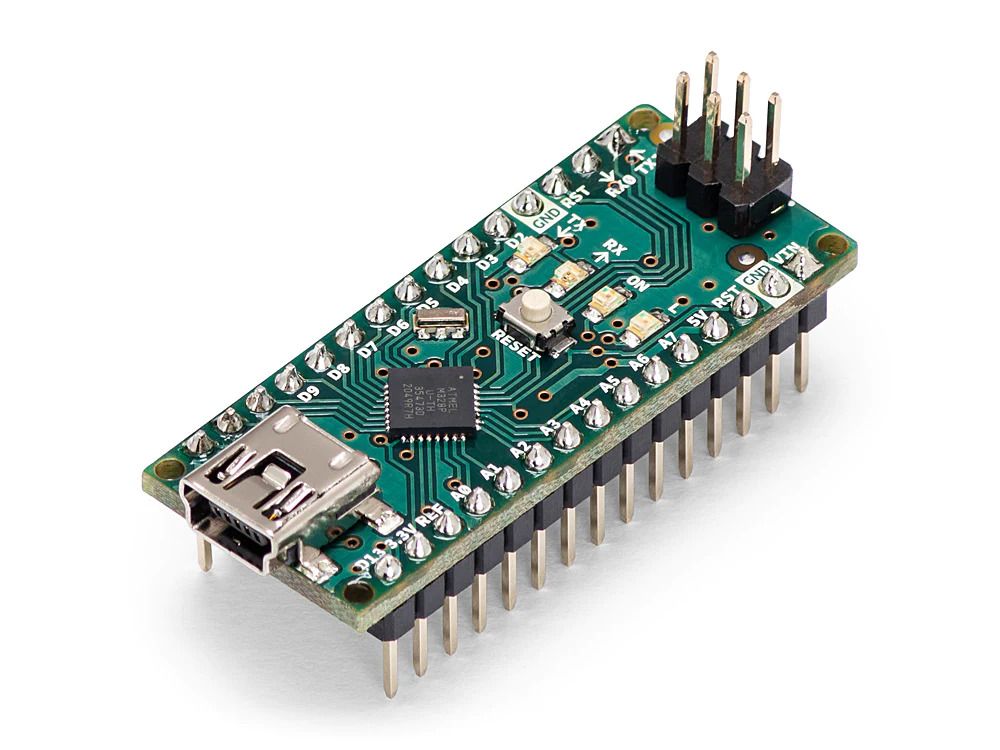
\includegraphics[height=2cm]{microcontroller/arduino/boards/nano.jpg}
                \caption{Arduino\textregistered{} Nano (\textit{Nano Family})}
            \end{figure}
            \begin{figure}
                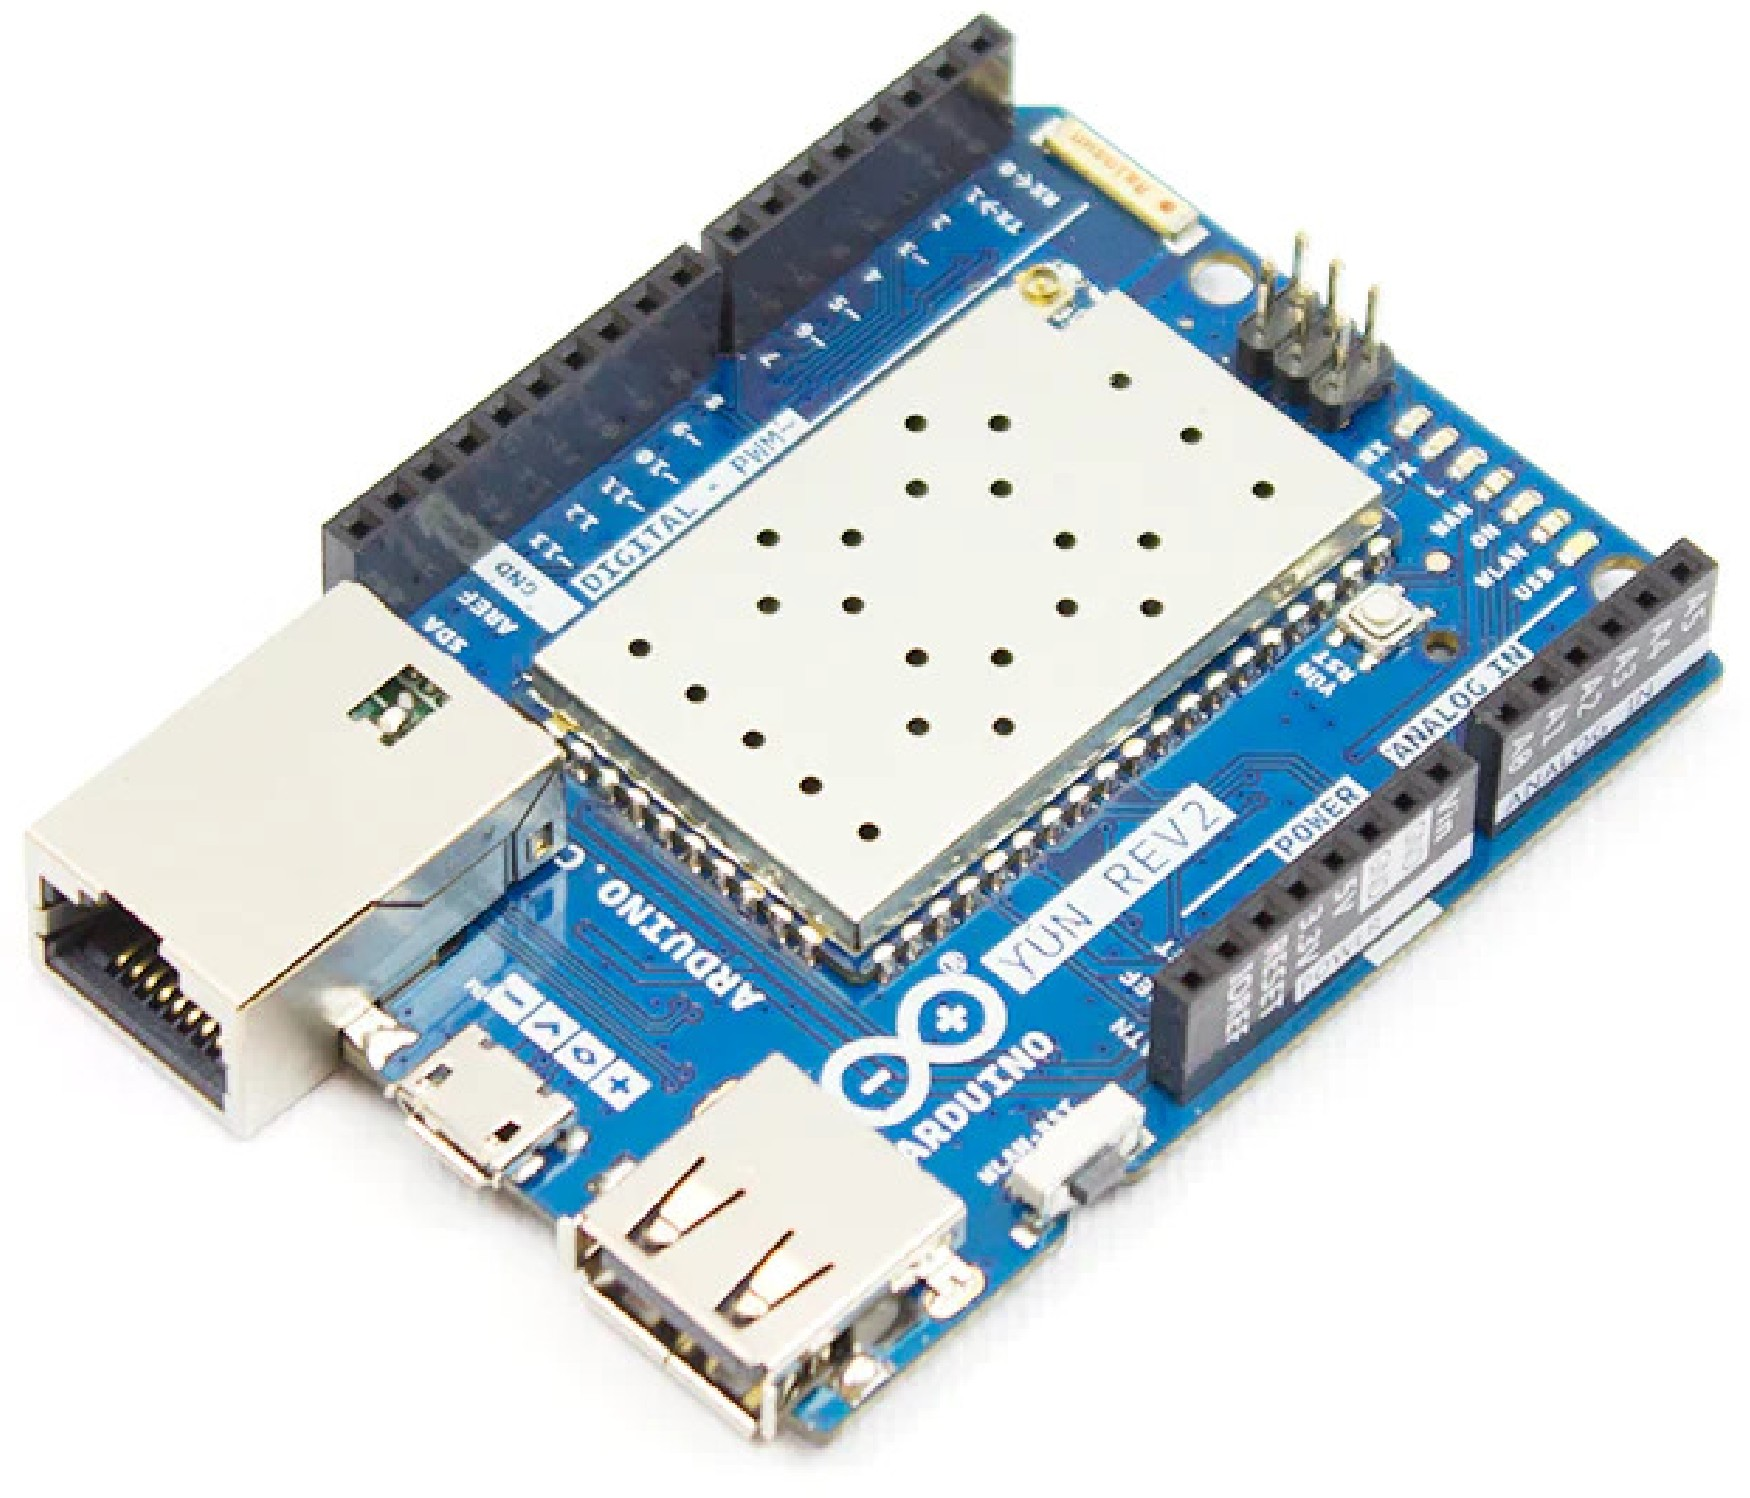
\includegraphics[height=2.7cm]{microcontroller/arduino/boards/yun.jpg}
                \caption{Arduino\textregistered{} Yún (\textit{Classic})}
            \end{figure}
        \end{column}
        \begin{column}{0.5\textwidth}
            \begin{figure}
                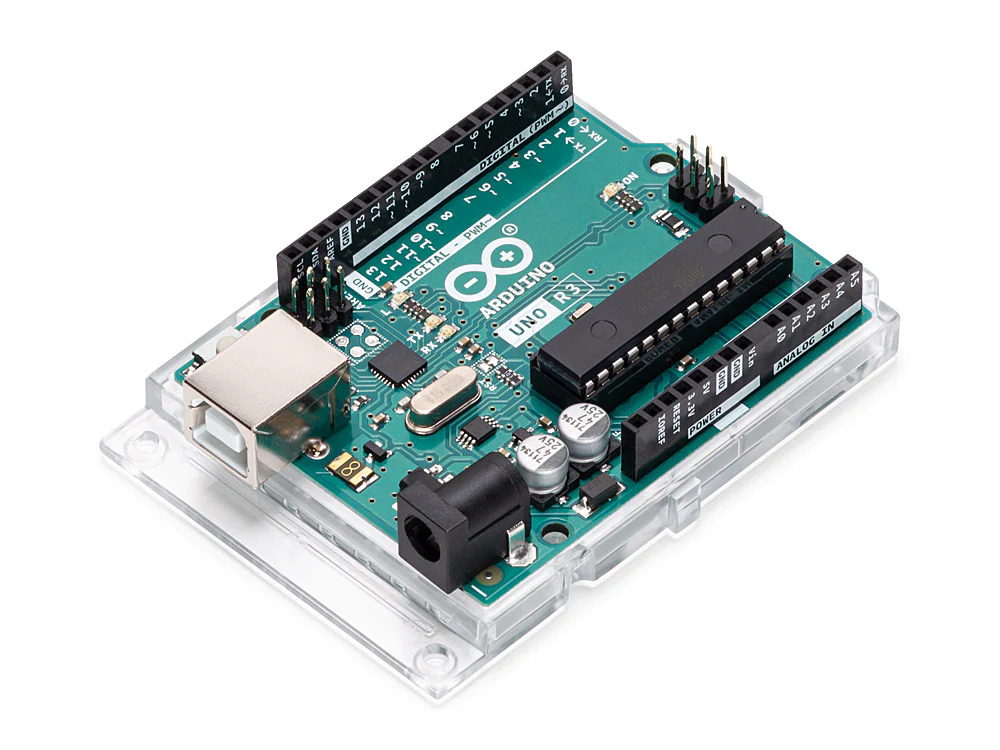
\includegraphics[height=2.7cm]{microcontroller/arduino/boards/uno.jpg}
                \caption{Arduino\textregistered{} Uno (\textit{Classic})}
            \end{figure}
            \begin{figure}
                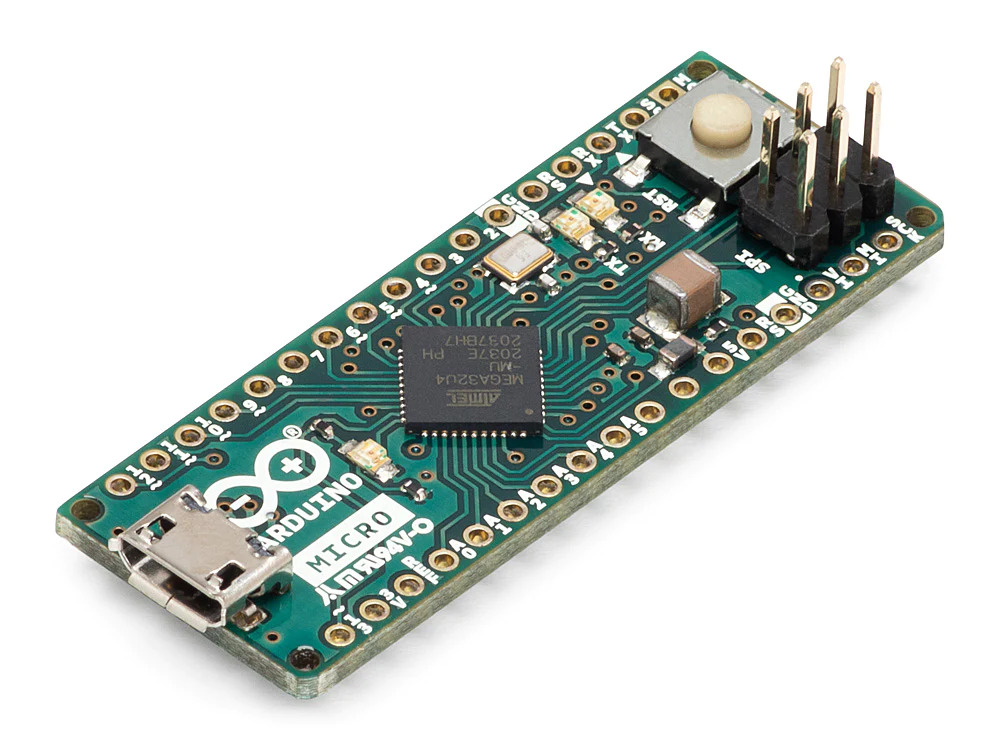
\includegraphics[height=2cm]{microcontroller/arduino/boards/micro.jpg}
                \caption{Arduino\textregistered{} Micro (\textit{Classic})}
            \end{figure}
        \end{column}
    \end{columns}
\end{frame}

\begin{frame}
    % \par Different board examples:
    \begin{columns}
        \begin{column}{0.5\textwidth}
            \begin{figure}
                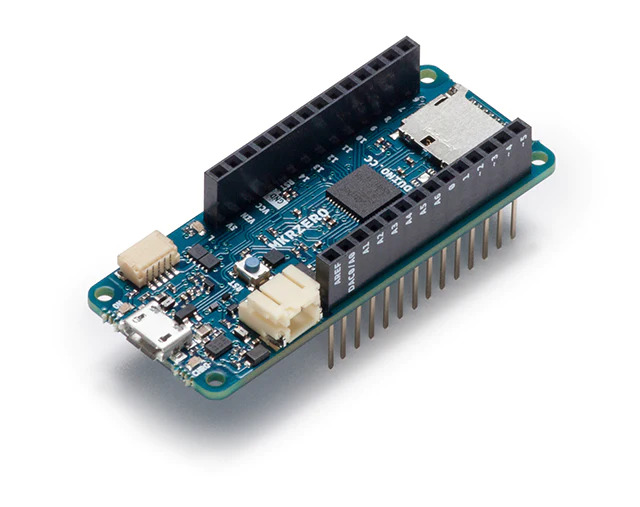
\includegraphics[height=2cm]{microcontroller/arduino/boards/mkr-zero.jpg}
                \caption{Arduino\textregistered{} MKR ZERO (\textit{MKR Family})}
            \end{figure}
            \begin{figure}
                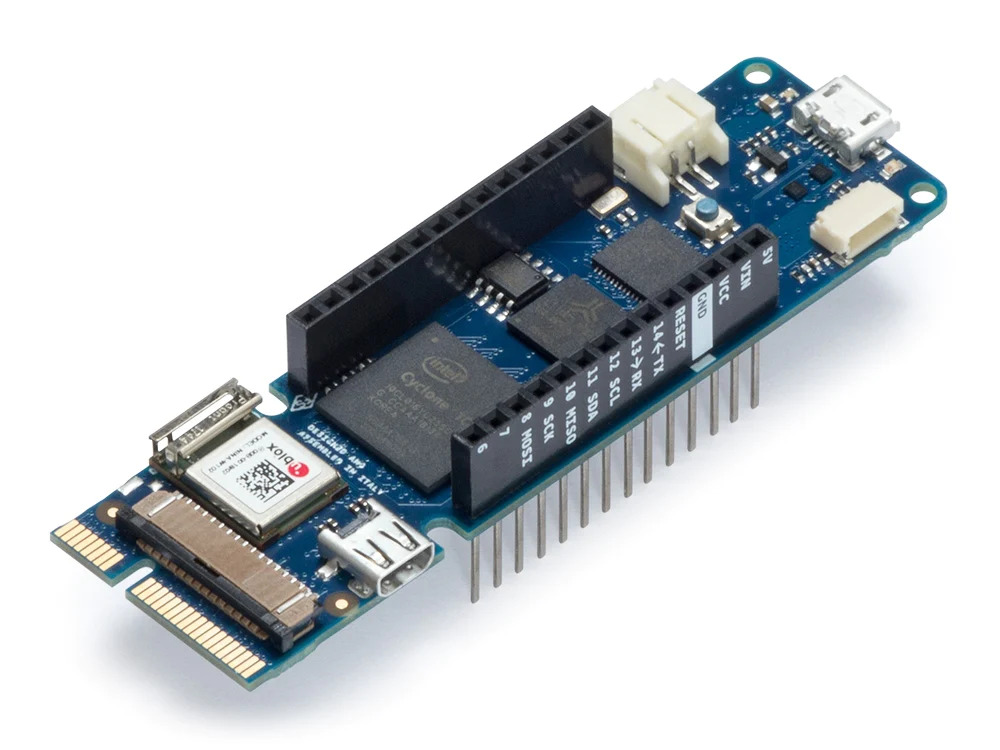
\includegraphics[height=2cm]{microcontroller/arduino/boards/mkr-vidor-4000.jpg}
                \caption{Arduino\textregistered{} MKR Vidor 4000 (\textit{MKR Family})}
            \end{figure}
        \end{column}
        \begin{column}{0.5\textwidth}
            \begin{figure}
                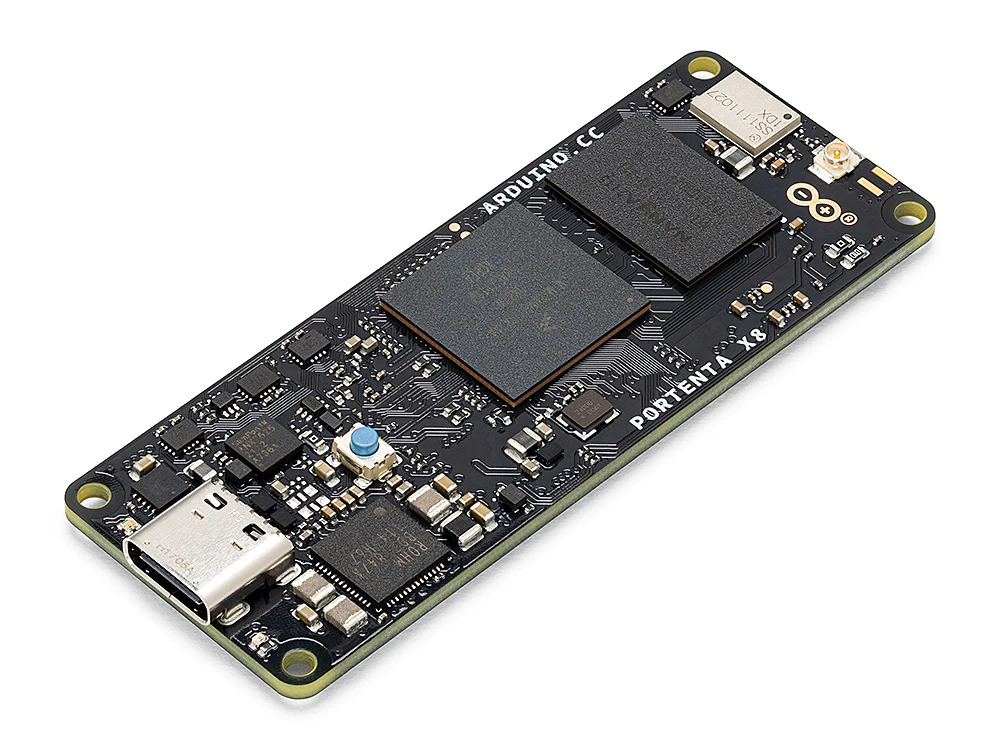
\includegraphics[height=2cm]{microcontroller/arduino/boards/portenta-x8.jpg}
                \caption{Arduino\textregistered{} Portenta X8 (\textit{Portenta Family})}
            \end{figure}
            \begin{figure}
                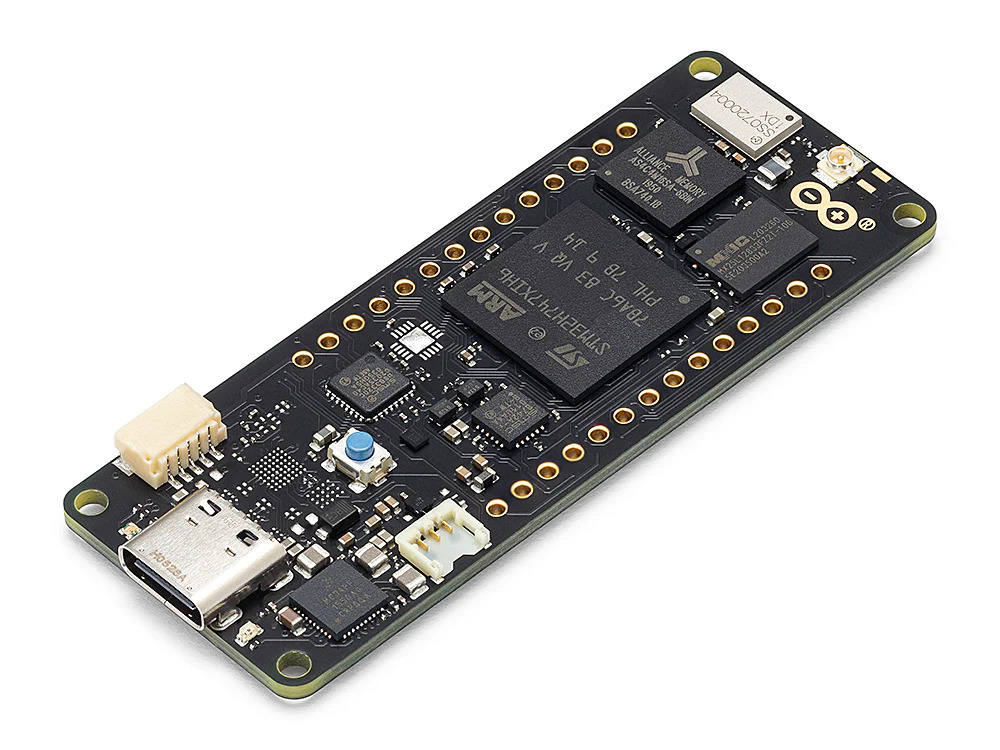
\includegraphics[height=2cm]{microcontroller/arduino/boards/portenta-h7-lite-connected.jpg}
                \caption{Arduino\textregistered{} Portenta H7 Lite Connected (\textit{Portenta Family})}
            \end{figure}
        \end{column}
    \end{columns}
\end{frame}

\subsection{Shields}
\begin{frame}
    \begin{columns}
        \begin{column}{0.5\textwidth}
            \begin{figure}
                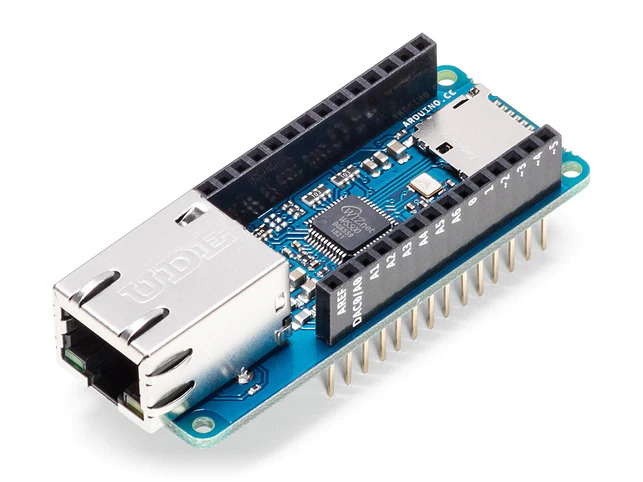
\includegraphics[height=2cm]{microcontroller/arduino/shields/mkr-ethernet-shield.jpg}
                \caption{Arduino\textregistered{} MKR \glsentrytext{eth} Shield}
            \end{figure}
            \begin{figure}
                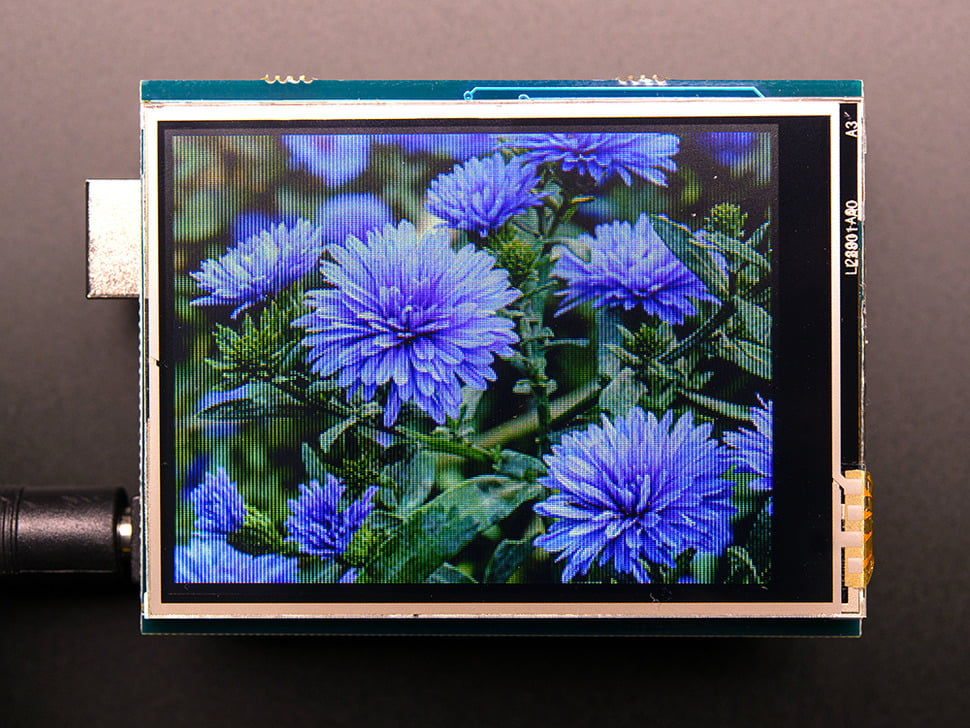
\includegraphics[height=2cm]{microcontroller/arduino/shields/adafruit-tft-touch-shield.jpg}
                \caption{Adafruit \glsentrytext{tft} Touch Shield for Arduino\textregistered{}}
            \end{figure}
        \end{column}
        \begin{column}{0.5\textwidth}
            \begin{figure}
                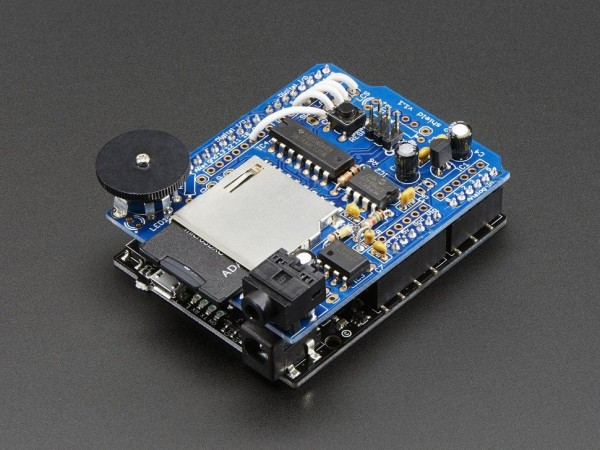
\includegraphics[height=2cm]{microcontroller/arduino/shields/adafruit-wave-shield.jpg}
                \caption{Adafruit Wave Shield for Arduino\textregistered{} Kit}
            \end{figure}
            \begin{figure}
                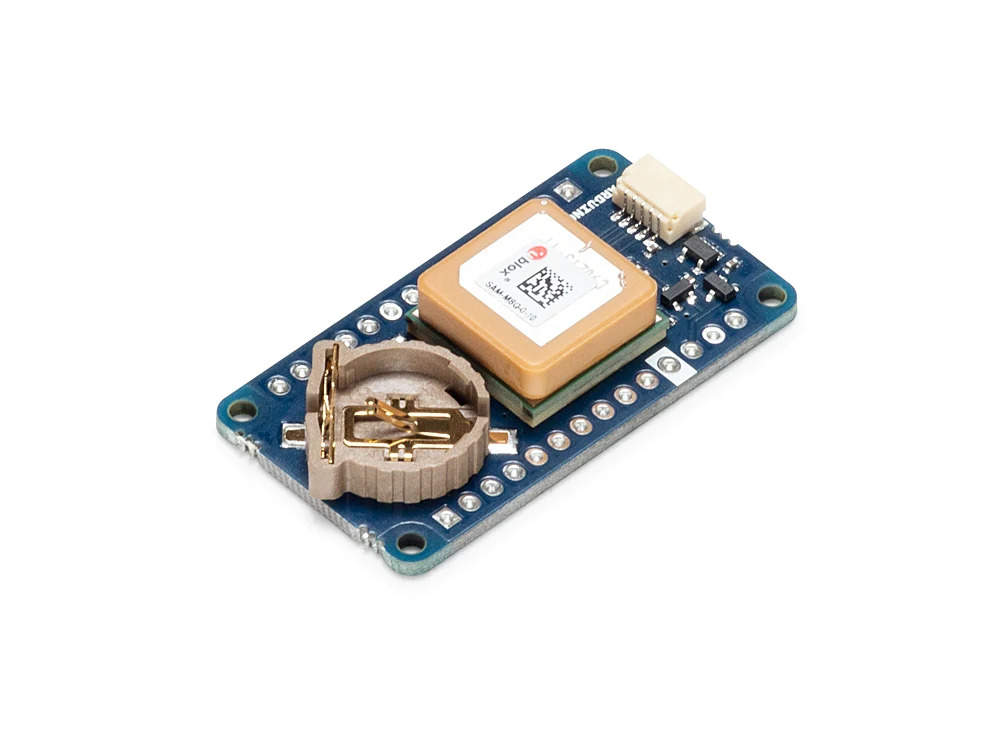
\includegraphics[height=2cm]{microcontroller/arduino/shields/mkr-gps-shield.jpg}
                \caption{Arduino\textregistered{} MKR \glsentrytext{gps} Shield}
            \end{figure}
        \end{column}
    \end{columns}
\end{frame}

\subsection{Sensors}

\begin{frame}
    \begin{columns}
        \begin{column}{0.5\textwidth}
            % \par 3-axis Accelerometer
            \begin{figure}
                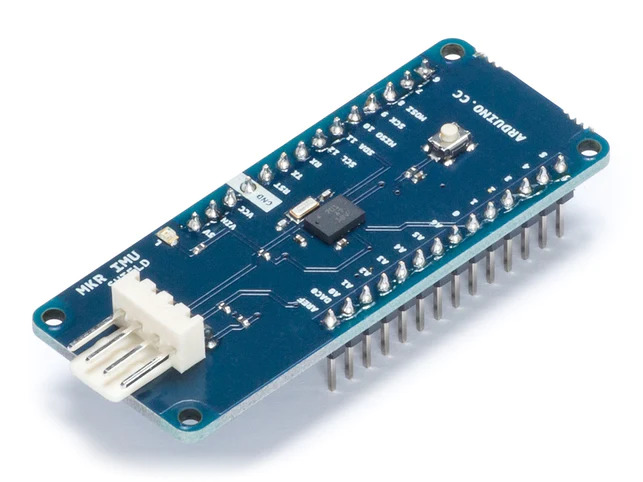
\includegraphics[height=2cm]{microcontroller/arduino/shields/mkr-imu-shield.jpg}
                \caption{Arduino\textregistered{} MKR \glsentrytext{imu} Shield}
            \end{figure}
            % \par Proximity Sensors
            \begin{figure}
                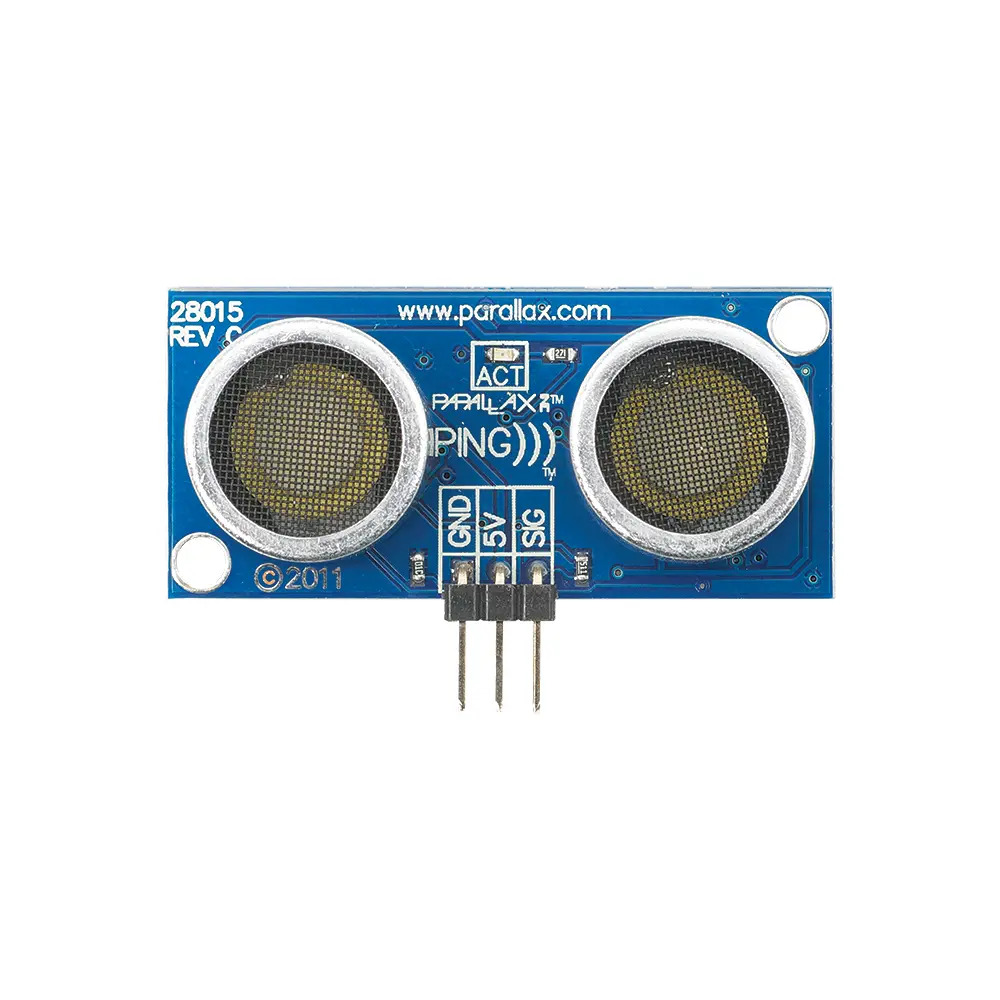
\includegraphics[height=3cm]{microcontroller/sensors/parallax-ultrasonic-proximity-sensor.jpg}
                \caption{\href{https://www.parallax.com/product/ping-ultrasonic-distance-sensor/}{Parralax Ultrasonic Proximity Sensor} (up to \SI{8}{\meter})}
            \end{figure}
        \end{column}
        \begin{column}{0.5\textwidth}
            % \par Resistive Force Sensor
            \begin{figure}
                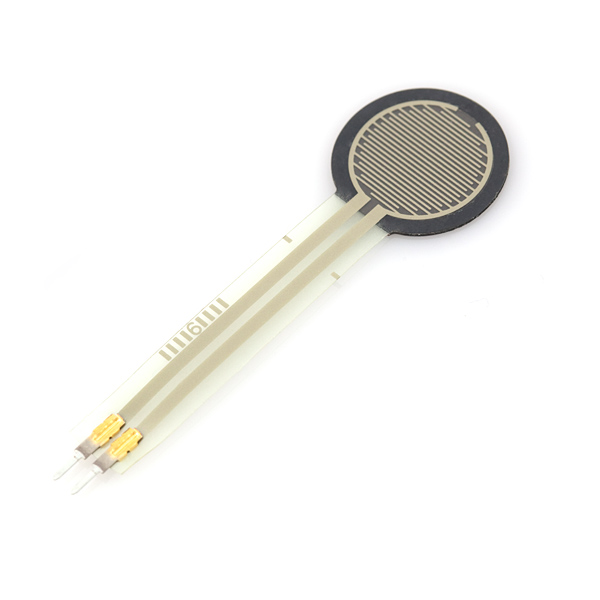
\includegraphics[height=2cm]{microcontroller/sensors/interlink-electronics-force-sensitive-sensor.jpg}
                \caption{\href{https://cdn.sparkfun.com/assets/8/a/1/2/0/2010-10-26-DataSheet-FSR402-Layout2.pdf}{Interlink Electronics Force Sensitive Sensor}}
            \end{figure}
            % Sharp GP2Y0A21YK
            \begin{figure}
                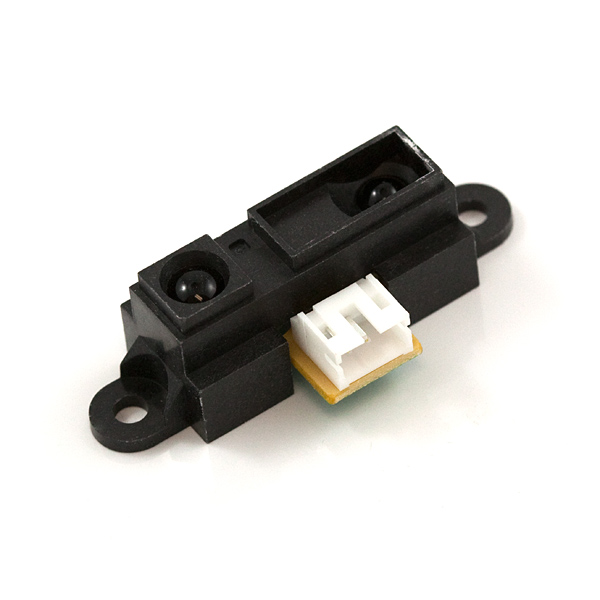
\includegraphics[height=3cm]{microcontroller/sensors/sharp-infrared-proximity-sensor.jpg}
                \caption{Sharp \glsentrytext{ir} Proximity Sensor: \href{https://global.sharp/products/device/lineup/data/pdf/datasheet/gp2y0a21yk\_e.pdf}{GP2Y0A21YK0F} (up to \SI{1}{\meter})}
            \end{figure}
        \end{column}
    \end{columns}
\end{frame}

\subsection{Actuators}

\begin{frame}
    \begin{columns}[t]
        \begin{column}{0.5\textwidth}
            % \par Hydraulic or pneumatic cylinders and valves
            \begin{figure}
                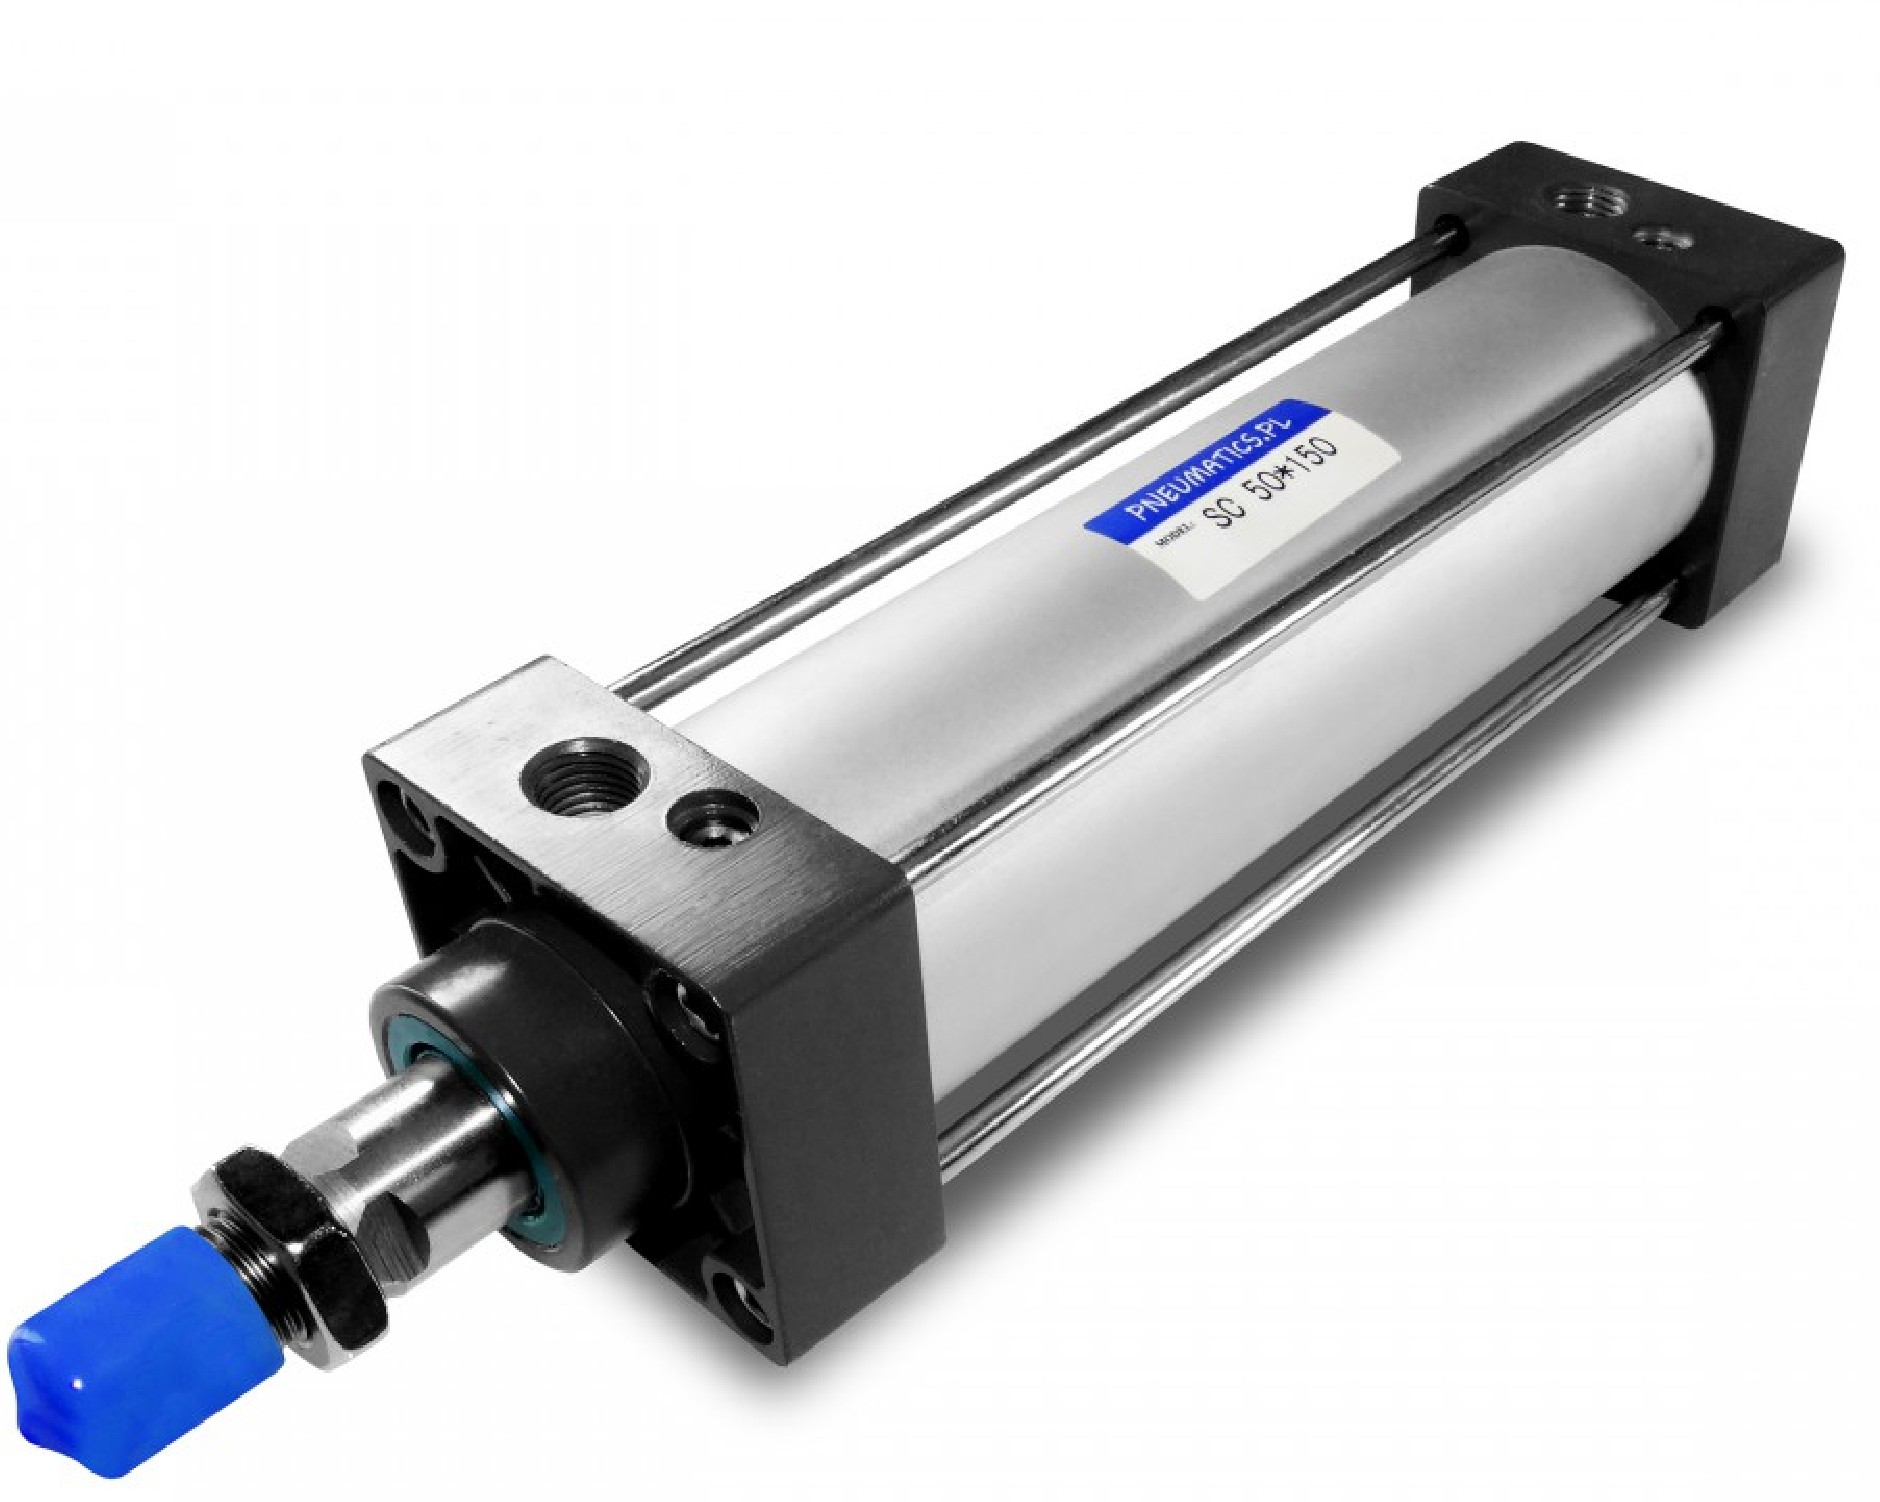
\includegraphics[height=2.5cm]{microcontroller/actuators/pneumatic-cylinder-drive.jpg}
                \caption{\href{https://hpcontrol.eu/silownik-pneumatyczny-naped-32x200-sc.html}{Hydraulic or Pneumatic Cylinders and Valves}}
            \end{figure}
        \end{column}
        \begin{column}{0.5\textwidth}
            % \par Relais
            \begin{figure}
                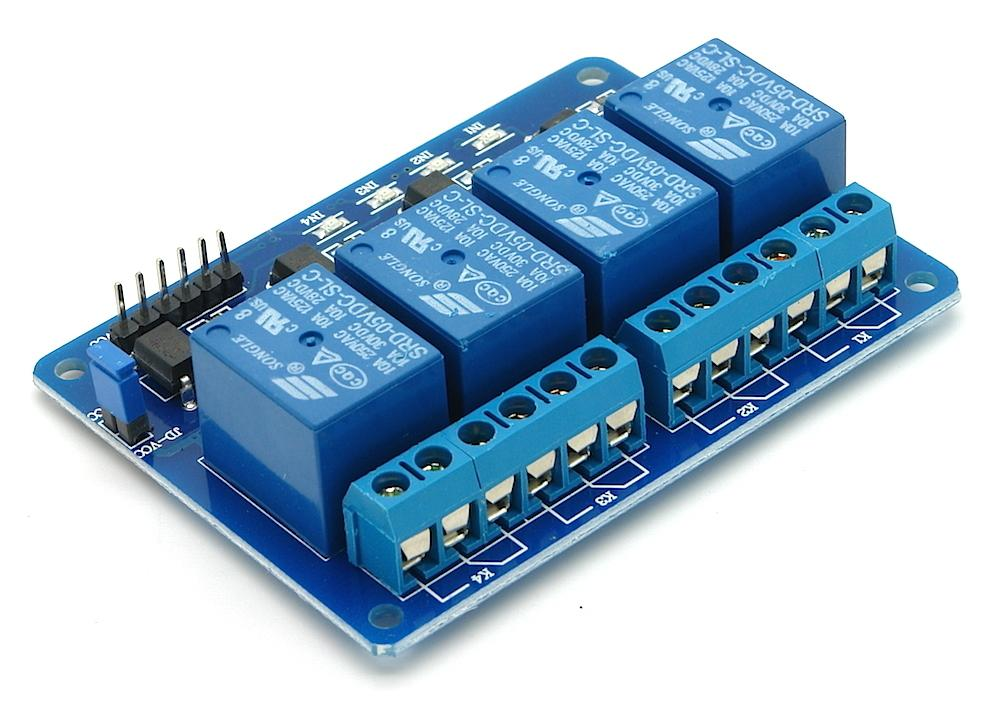
\includegraphics[height=2.5cm]{microcontroller/actuators/sertronics-relais-52975.jpg}
                \caption{\href{https://b2b.sertronics-shop.de/Sensoren-/-Module/Relaiskarten/5V-4-Kanal-Relais-Modul/}{Sertronics 4 Channel Relay Module}}
            \end{figure}
        \end{column}
    \end{columns}
    % \par \acs{lcd}
    \begin{figure}
        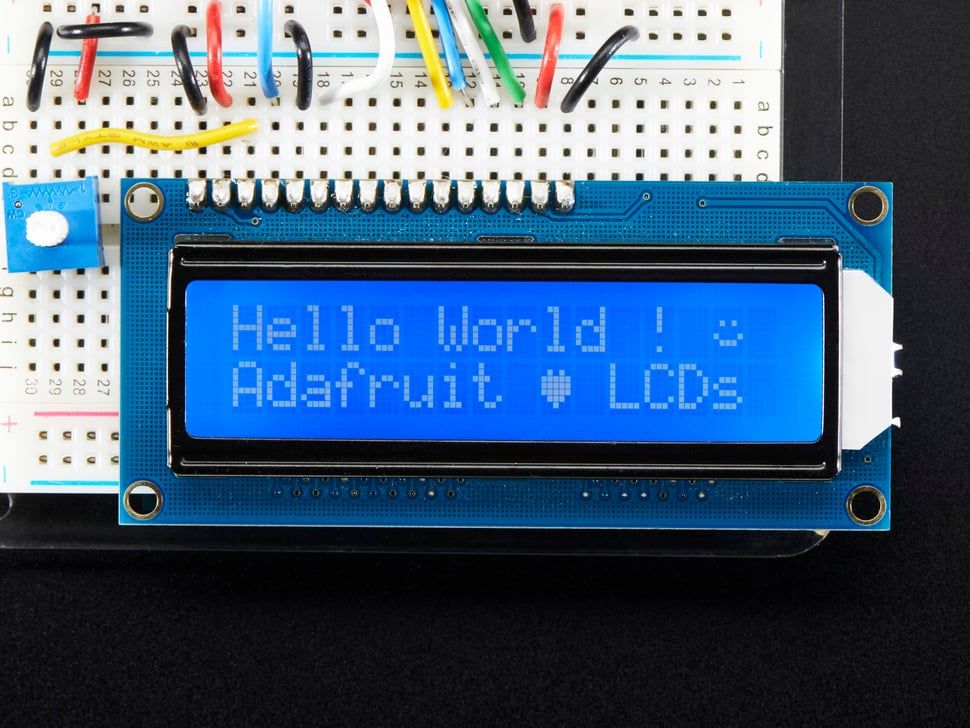
\includegraphics[height=2.5cm]{microcontroller/actuators/adafruit-lcd.jpg}
        \caption{\href{https://www.adafruit.com/product/181}{Adafruit Standard HD44780} \glsentrytext{lcd}s}
    \end{figure}
\end{frame}

\begin{frame}
    % \begin{columns}
    %     \begin{column}{0.5\textwidth}
    % \par Solenoids/Valves
    \begin{figure}
        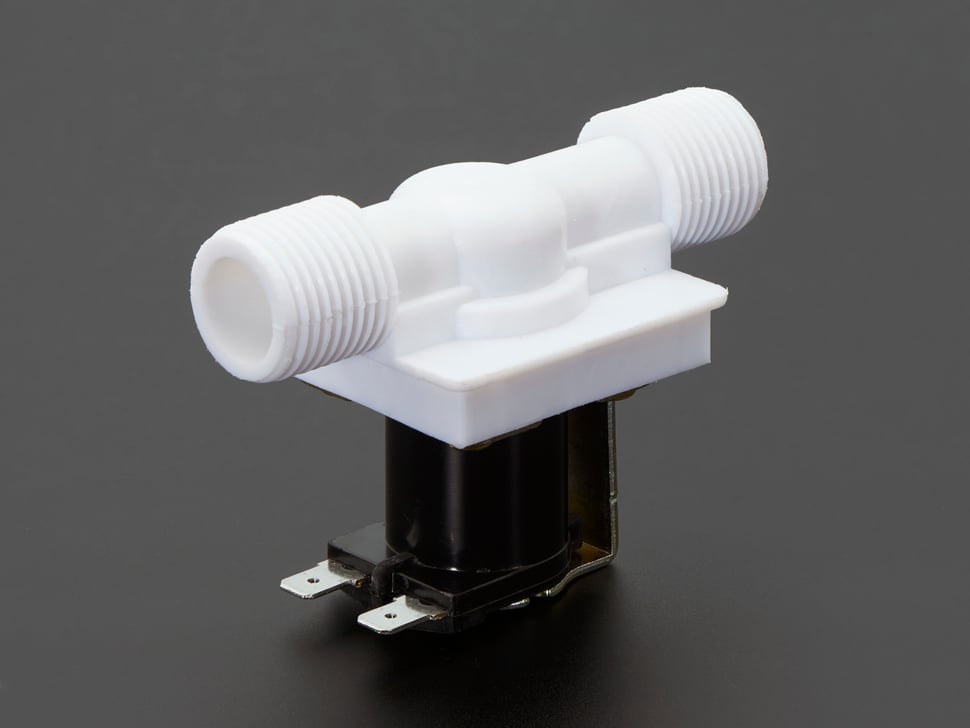
\includegraphics[height=3cm]{microcontroller/actuators/adafruit-water-solenoid-valve.jpg}
        \caption{\href{https://www.adafruit.com/product/997}{Adafruit Plastic Water Solenoid Valve}}
    \end{figure}
    % \end{column}
    % \begin{column}{0.5\textwidth}
    % \par Stepper Motors
    \begin{figure}
        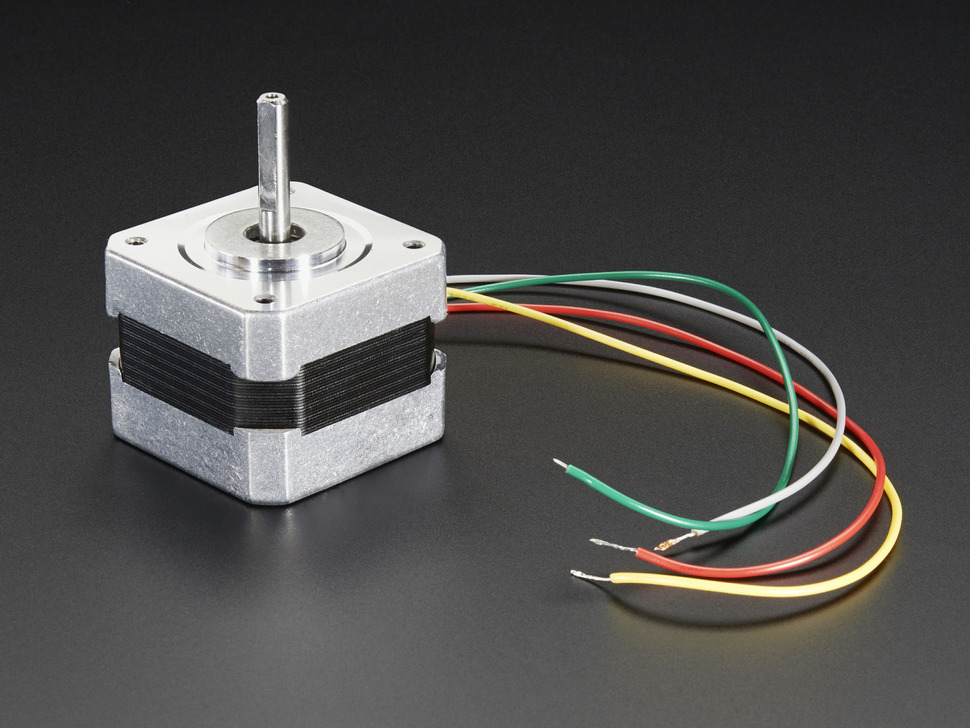
\includegraphics[height=3cm]{microcontroller/actuators/adafruit-stepper-motor-nema-17.jpg}
        \caption{\href{https://www.adafruit.com/product/324}{Adafruit Stepper Motor}}
    \end{figure}
    %     \end{column}
    % \end{columns}
\end{frame}

% \begin{frame}{Resources}
%     \begin{itemize}
%         \item \href{https://docs.arduino.cc/learn/starting-guide/getting-started-arduino}{Getting Started with Arduino}
%     \end{itemize}
% \end{frame}

\section{Arduino\textregistered{} Nano RP2040 Connect}

\begin{frame}
    \begin{itemize}
        \item Compact development board based on the RP2040 microcontroller
        \item Dual-core \acs{arm} Cortex-M0+ processor with a clock speed of \SI{133}{\mega\hertz}
        \item \SI{2}{\mebi\byte} of onboard flash memory
        \item Integrated \acs{wifi} and \ac{ble} connectivity
        \item 6-axis \ac{imu} for motion sensing
        \item Built-in microphone for audio input
        \item U-blox NINA-W102 module for wireless connectivity
    \end{itemize}
    \begin{figure}
        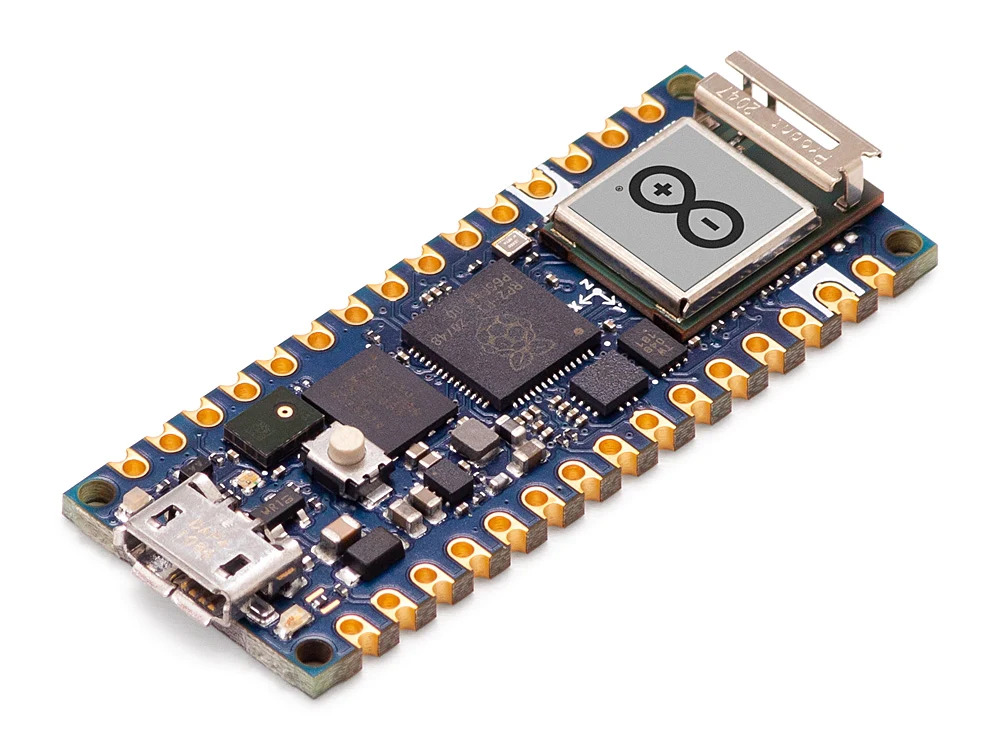
\includegraphics[height=2cm]{microcontroller/arduino/rp2040/rp2040-connect-isometric.jpg}
        \caption{Arduino\textregistered{} Nano RP2040 Connect: Board}
    \end{figure}
\end{frame}

\subsection{Pinout}
\begin{frame}
    \begin{figure}
        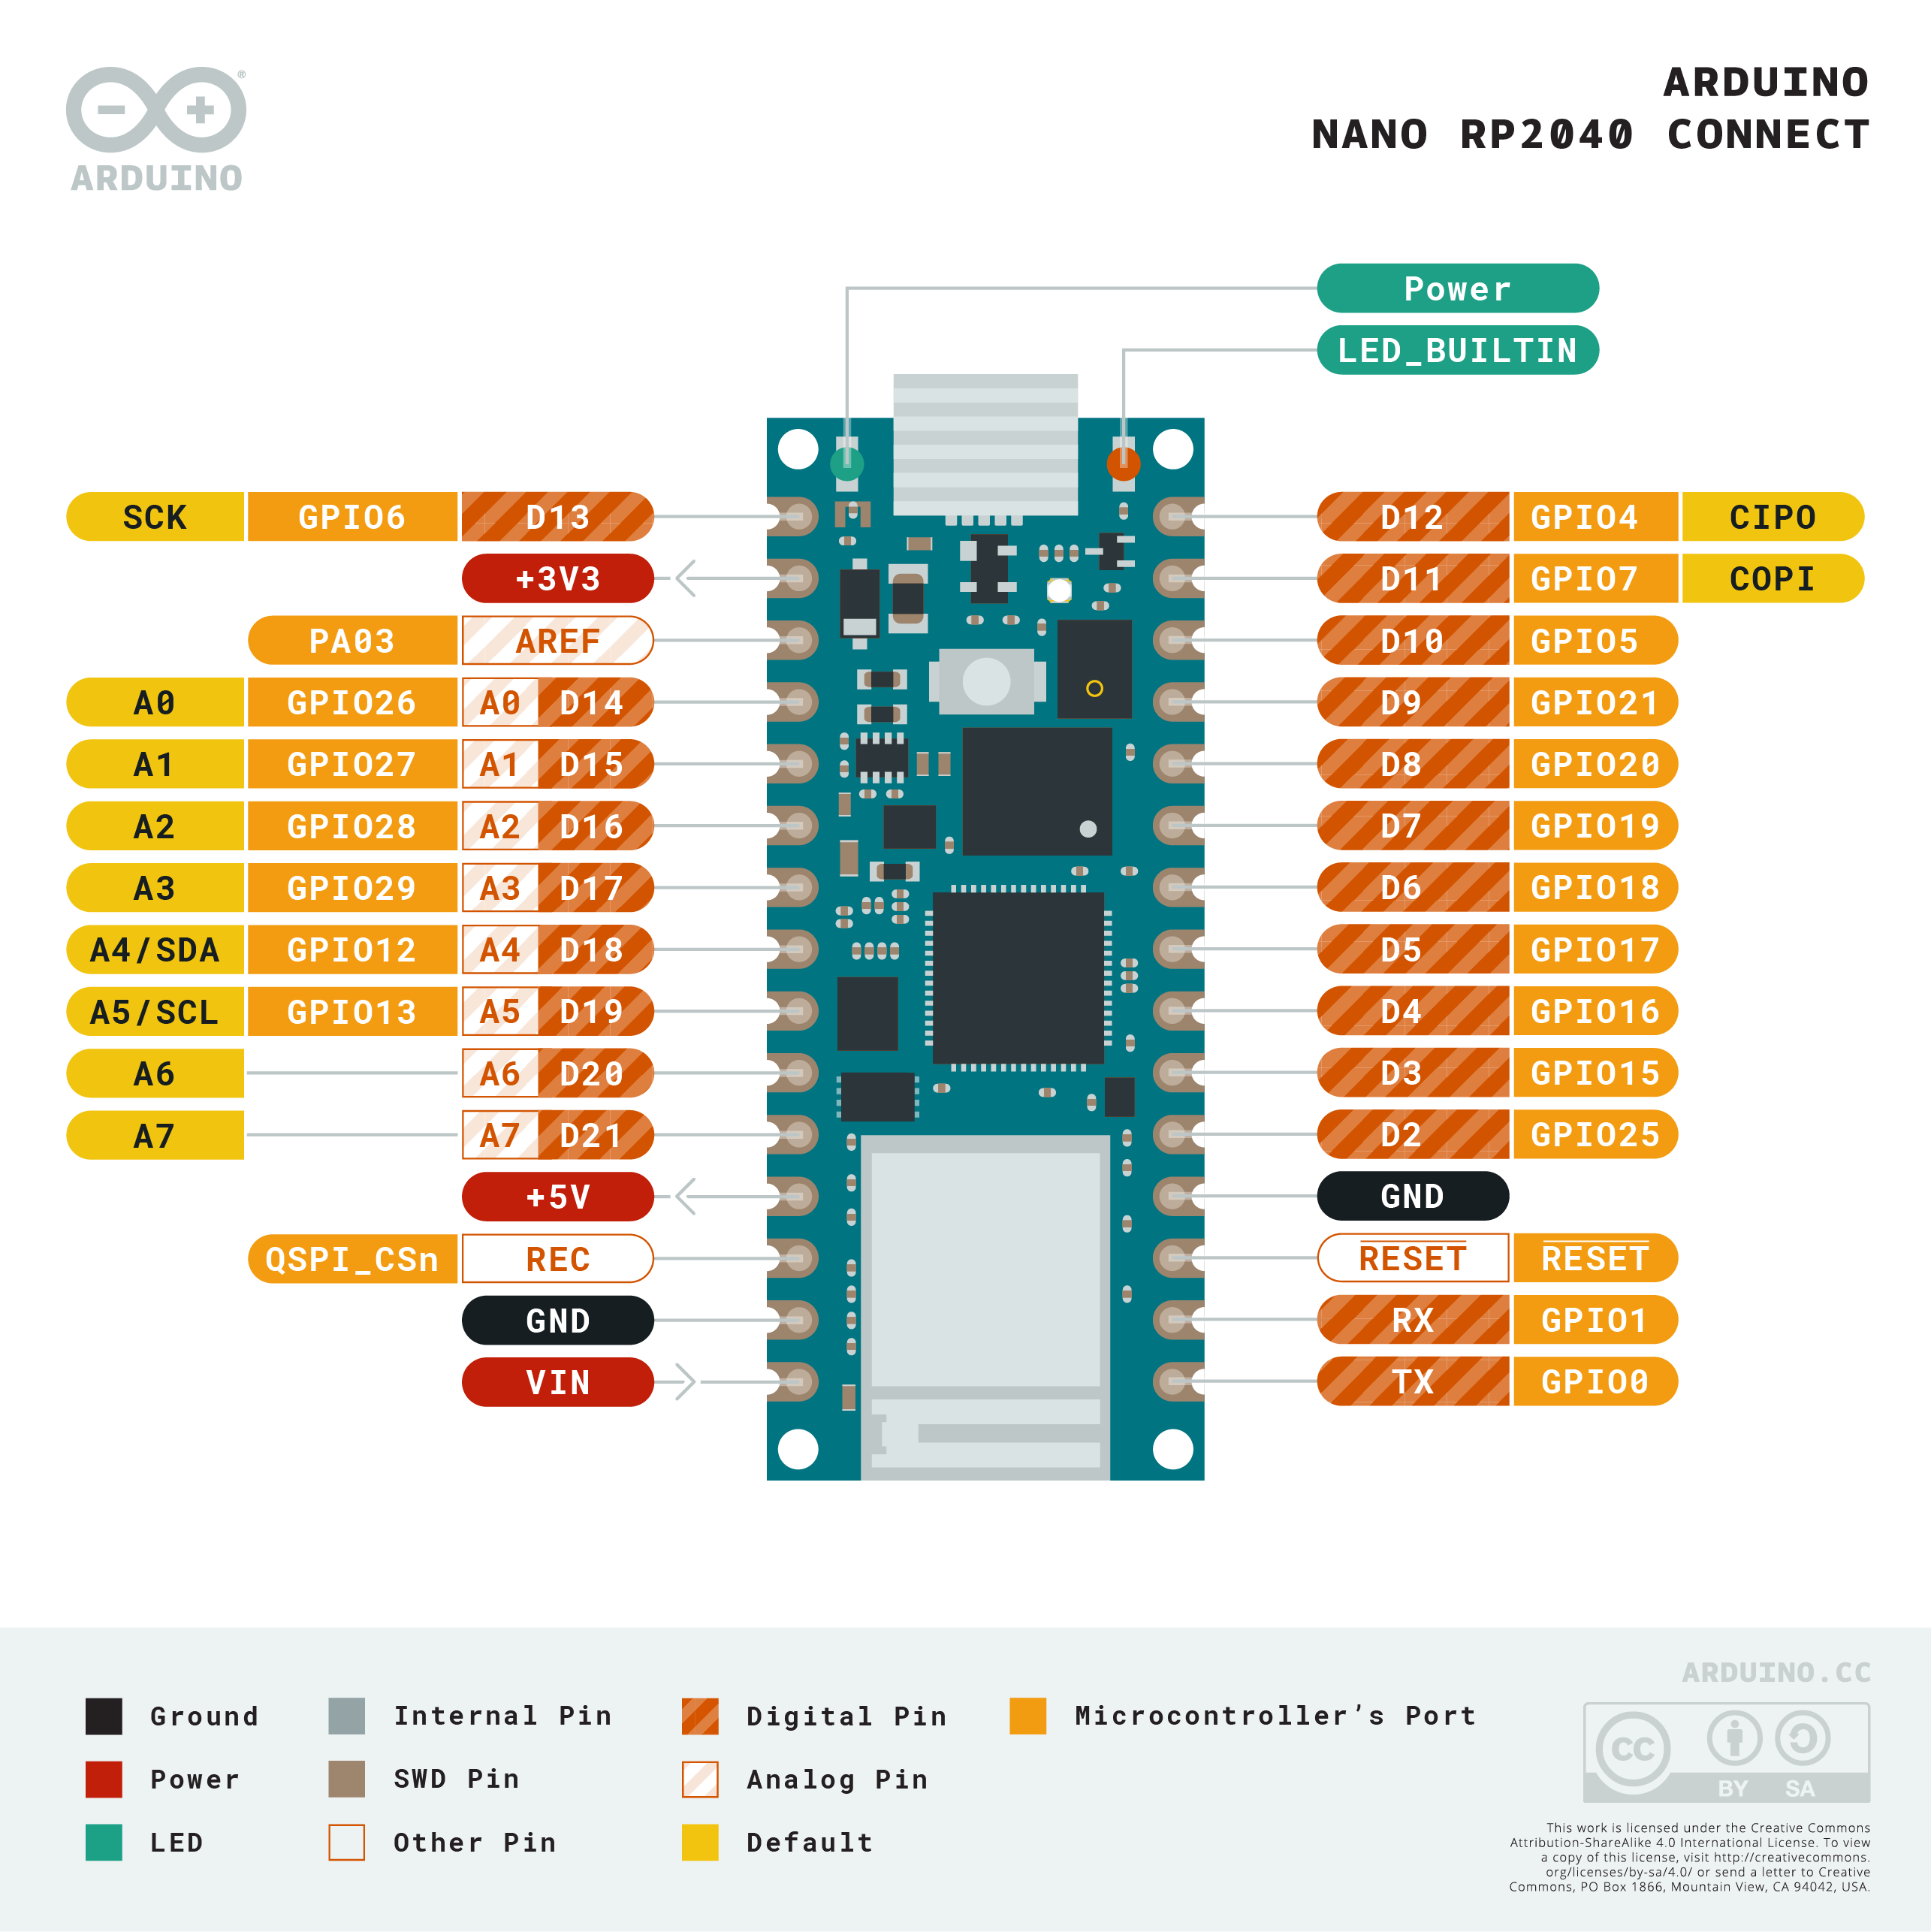
\includegraphics[width=0.9\textwidth]{microcontroller/arduino/rp2040/pinout.png}
        \caption{Arduino\textregistered{} Nano RP2040 Connect: Pinout}
    \end{figure}
\end{frame}

\subsection{Schematic}
\begin{frame}
    \begin{figure}
        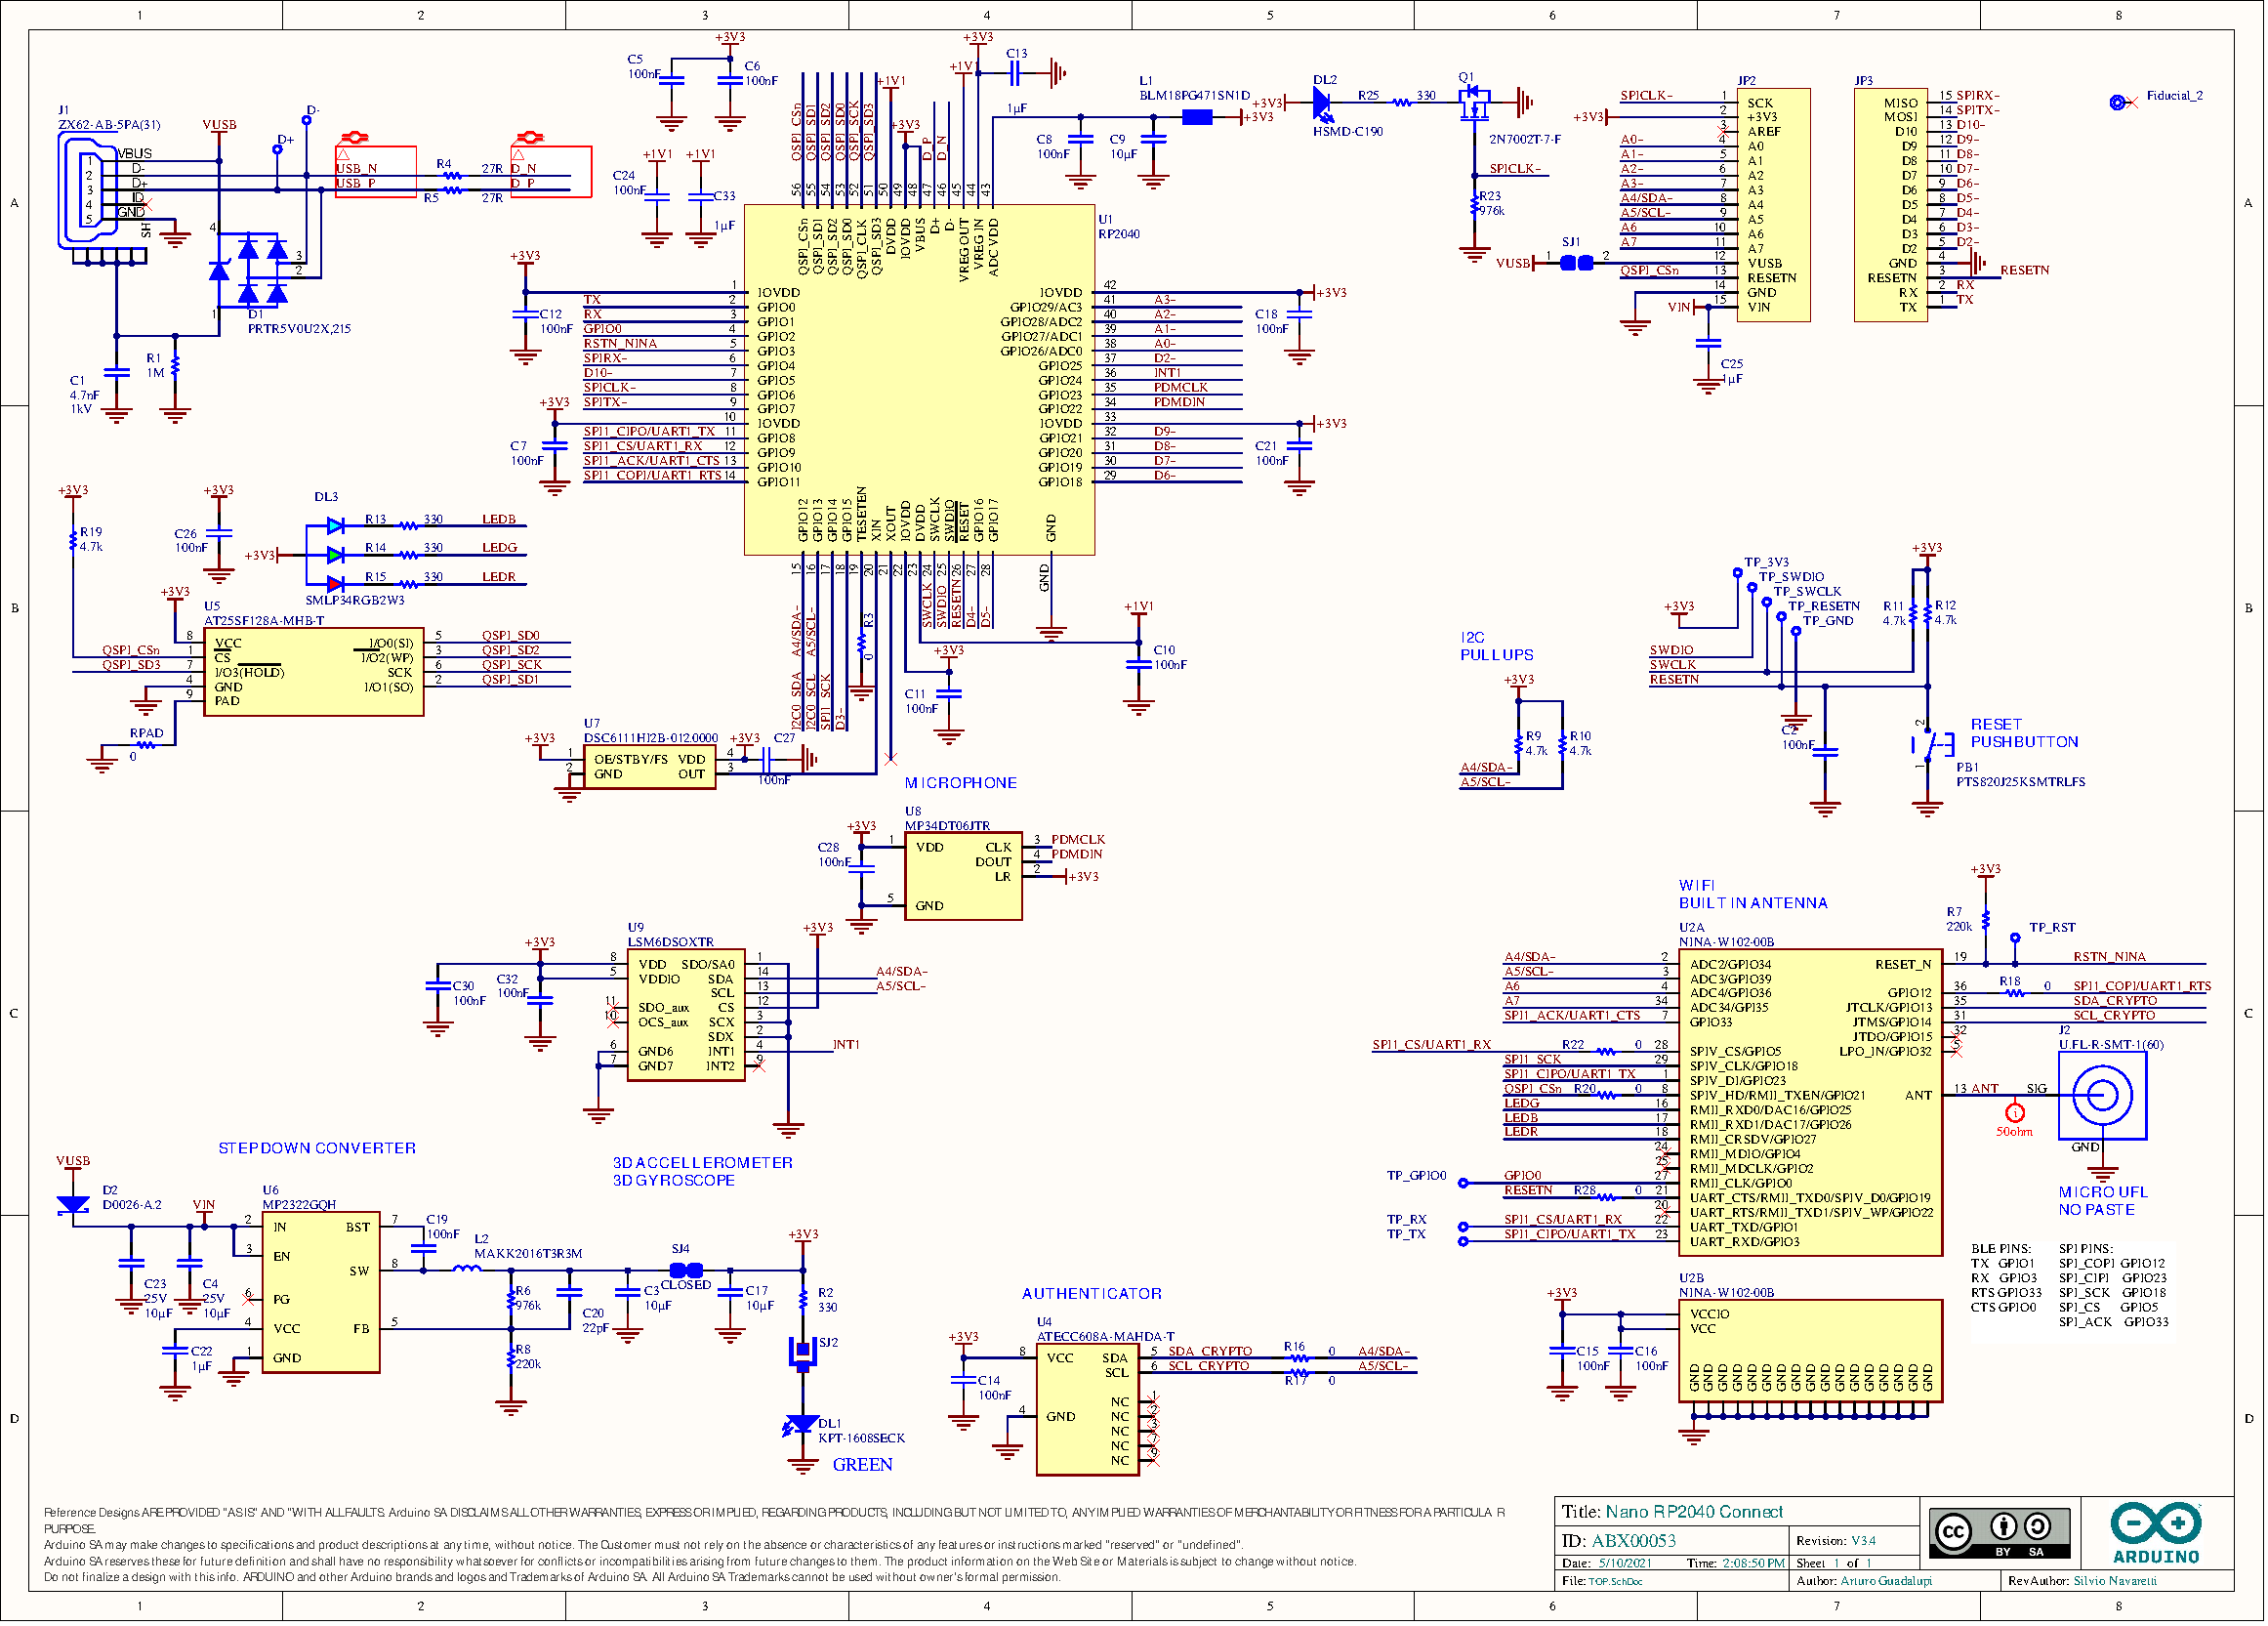
\includegraphics[width=0.9\textwidth]{microcontroller/arduino/rp2040/schematic.pdf}
        \caption{Arduino\textregistered{} Nano RP2040 Connect: Schematic}
    \end{figure}
\end{frame}

\subsection{Resources}
\begin{frame}
    \begin{itemize}
        \item General
              \begin{itemize}
                  \item \href{https://content.arduino.cc/assets/ABX00053-datasheet.pdf}{Arduino\textregistered{} Nano RP2040 Connect: Datasheet}
                  \item \href{https://content.arduino.cc/assets/Pinout\_NanoRP2040\_latest\%20\%281\%29.png}{Arduino\textregistered{} Nano RP2040 Connect: Pinout}
                  \item \href{https://content.arduino.cc/assets/ABX00053-schematics.pdf}{Arduino\textregistered{} Nano RP2040 Connect: Schematic}
                  \item \href{https://docs.arduino.cc/tutorials/nano-rp2040-connect/rp2040-01-technical-reference}{Arduino\textregistered{} Nano RP2040 Connect: C Cheatsheet}
                  \item \href{https://docs.arduino.cc/tutorials/nano-rp2040-connect/rp2040-python-api}{Arduino\textregistered{} Nano RP2040 Connect: Python\textregistered{} \acs{api} Guide}
                        %   \item \href{https://store.arduino.cc/products/arduino-nano-rp2040-connect\#docs}{Arduino\textregistered{} Interactive Board Viewer}
              \end{itemize}
        \item \acsp{ic}
              \begin{itemize}
                  \item \href{https://datasheets.raspberrypi.com/rp2040/rp2040-datasheet.pdf}{Raspberry Pi RP2040 Microcontroller}
                  \item \href{https://content.u-blox.com/sites/default/files/NINA-W10\_DataSheet\_UBX-17065507.pdf}{U-blox\textregistered{} Nina W102 \acs{wifi}/Bluetooth Module}
                  \item \href{https://ww1.microchip.com/downloads/en/DeviceDoc/40001977A.pdf}{Microchip\textregistered{} ATECC608A Crypto}
                  \item \href{https://www.renesas.com/in/en/document/dst/at25sf128a-datasheet?r=1608781}{AT25SF128A \SI{16}{\mebi\byte} NOR Flash}
                  \item \href{https://www.st.com/resource/en/datasheet/mp34dt06j.pdf}{ST MP34DT06JTR \glsentrydesc{mems} Microphone}
                  \item \href{https://www.st.com/resource/en/datasheet/lsm6dsox.pdf}{ST LSM6DSOXTR 6-axis \glsentrytext{imu}}
              \end{itemize}
        \item \aclp{sdk}/\aclp{os}
              \begin{itemize}
                  \item C/C++: \href{https://github.com/arduino/ArduinoCore-mbed/releases/tag/2.0.0}{Arduino\textregistered{} Core Mbed}, \href{https://github.com/earlephilhower/arduino-pico}{Arduino\textregistered{} Pico}
                  \item Python: \href{https://micropython.org/download/ARDUINO\_NANO\_RP2040\_CONNECT/}{MicroPython}, \href{https://github.com/openmv/openmv/releases}{Open\glsentrytext{mv} MicroPython}, \href{https://circuitpython.org/board/arduino\_nano\_rp2040\_connect/}{Adafruit's CircuitPython}
              \end{itemize}
    \end{itemize}
\end{frame}

\section{Arduino\textregistered{} \glsentrytext{ide}}

\begin{frame}
    \begin{columns}
        \begin{column}{0.45\textwidth}
            \begin{figure}
                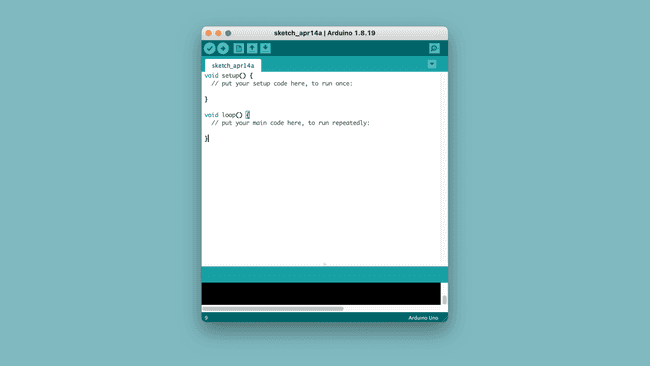
\includegraphics[height=2.6cm]{microcontroller/arduino/ide/ide-1.png}
                \caption{\href{https://www.arduino.cc/en/Guide}{Arduino\textregistered{} \glsentrytext{ide}} (\textit{Legacy})}
            \end{figure}
            \begin{figure}
                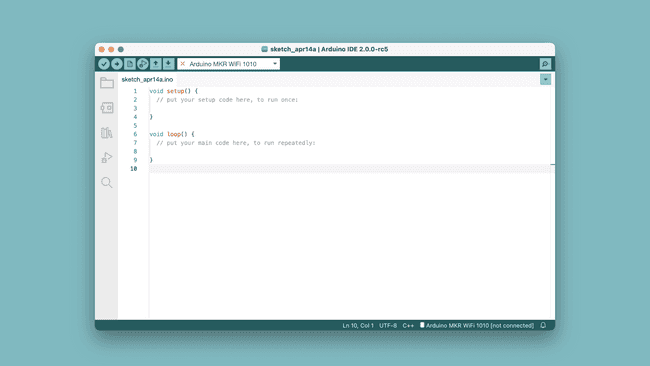
\includegraphics[height=2.6cm]{microcontroller/arduino/ide/ide-2.alt.png}
                \caption{\href{https://docs.arduino.cc/software/ide-v2/tutorials/getting-started-ide-v2}{Arduino\textregistered{} \glsentrytext{ide} 2.0}}
            \end{figure}
        \end{column}
        \begin{column}{0.55\textwidth}
            \begin{figure}
                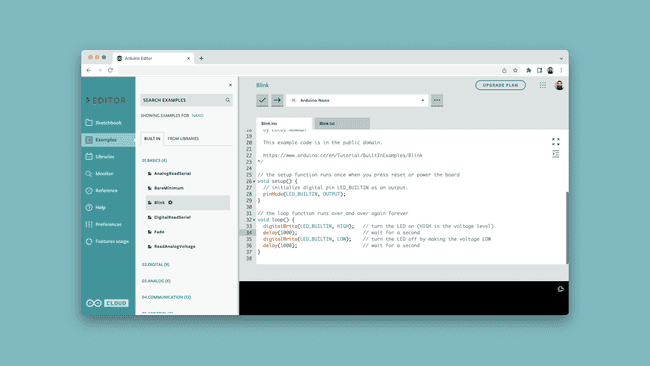
\includegraphics[height=2.6cm]{microcontroller/arduino/ide/web-editor.alt.png}
                \caption{\href{https://docs.arduino.cc/arduino-cloud/getting-started/getting-started-web-editor}{Arduino\textregistered{} Web Editor}}
            \end{figure}
            \begin{figure}
                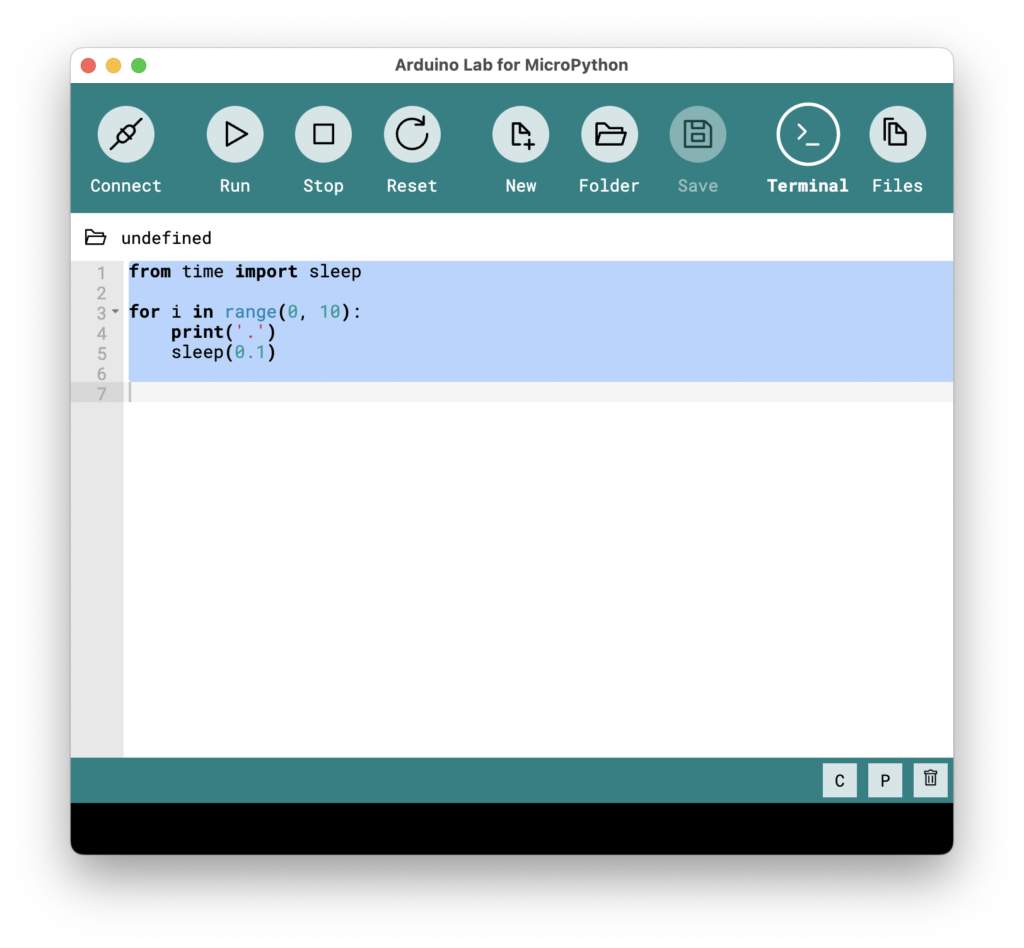
\includegraphics[height=2.6cm]{microcontroller/arduino/ide/arduino-lab-for-micropython.png}
                \caption{\href{https://docs.arduino.cc/micropython/}{Arduino\textregistered{} Lab for MicroPython}}
            \end{figure}
        \end{column}
    \end{columns}
\end{frame}

\begin{frame}{Program Structure}
    \par The Arduino\textregistered{} example ``Blink'' (see Listing \ref{lst:arduino:blinky}) is a simple and widely-used introductory program for Arduino\textregistered{} boards (cmp. ``Hello World'').
    \par It demonstrates the basic structure of Arduino\textregistered{} code, consisting of two primary functions, \mintinline{c}{setup()} and \mintinline{c}{loop()}.
    \begin{listing}[H]
        \inputsource[fontsize=\fontsize{8}{8}]{c}{arduino/blink.c}
        \caption{Arduino\textregistered{} example ``Blink''.}
        \label{lst:arduino:blinky}
    \end{listing}
\end{frame}

\begin{frame}{Program Structure}
    \par The \href{https://www.arduino.cc/reference/en/language/structure/sketch/setup/}{\mintinline{c}{setup()}} function runs once when you press reset or power the board.
    \par Inside of it, function \mintinline{c}{pinMode()} is used to configure the \ac{led} pin as an output.
    \begin{listing}[H]
        \inputsource[firstline=7,lastline=10]{c}{arduino/blink.c}
        \caption{Arduino\textregistered{} example ``Blink'': \mintinline{c}{setup()}}
        \label{lst:arduino:blinky:setup}
    \end{listing}
    \vspace{-1em}
    \par Function \href{https://www.arduino.cc/reference/en/language/functions/digital-io/pinmode/}{\mintinline{c}{pinMode(pin, mode)}} configures the specified \texttt{pin} either as an input or an output (\texttt{mode}).
    \par Many functions accept or expect predefined \href{https://www.arduino.cc/reference/en/language/variables/constants/constants/}{constants} or macros as parameter values (e.g. \mintinline[escapeinside=||]{c}{|\#|define LED_BUILTIN 13}).
\end{frame}

\begin{frame}{Program Structure}
    \par The \href{https://www.arduino.cc/reference/en/language/structure/sketch/loop/}{\mintinline{c}{loop()}} function runs over and over again forever.
    \par Functions \mintinline{c}{digitalWrite()} and \mintinline{c}{delay()} are used to toggle the \acs{led} and wait for a specific amount of time in between.
    \begin{listing}[H]
        \inputsource[fontsize=\fontsize{8}{8},firstline=13,lastline=18]{c}{arduino/blink.c}
        \caption{Arduino\textregistered{} example ``Blink'': \mintinline{c}{loop()}}
        \label{lst:arduino:blinky:loop}
    \end{listing}
    \vspace{-1em}
    \par Function \href{https://www.arduino.cc/reference/en/language/functions/digital-io/digitalwrite/}{\mintinline{c}{digitalWrite(pin, value)}} writes a \texttt{HIGH} or a \texttt{LOW} value to a digital \texttt{pin}.
    \par Function \href{https://www.arduino.cc/reference/en/language/functions/time/delay/}{\mintinline{c}{delay(ms)}} pauses the program for the amount of time (in milliseconds) specified.
\end{frame}

\section{Exercise I: Blink \glsentrytext{led} (onboard)}

\begin{frame}
    \begin{exampleblock}{Exercise I}
        \begin{enumerate}
            \item Get the Arduino\textregistered{} \acs{ide} of your choice.
            \item Connect your board to your \acs{pc}.
            \item Install the \ac{bsp} for your board.
            \item Run the example project ``Blink''.
            \item Extend the example project to log \texttt{On} and \texttt{Off} to the terminal.% of your \acs{pc} when toggling the \acs{led}.
        \end{enumerate}
        \par Hint:
        \begin{itemize}
            \item \href{https://www.arduino.cc/reference/en/language/functions/communication/serial/begin/}{\mintinline{c}{Serial.begin()}}
            \item \href{https://www.arduino.cc/reference/en/language/functions/communication/serial/println/}{\mintinline{c}{Serial.println()}}
        \end{itemize}
    \end{exampleblock}
\end{frame}

\begin{frame}{Solution: Exercise I}
    \begin{figure}
        \begin{tikzpicture}[circuitikz/bipoles/length=1cm]
            \draw (2,4) node[rp2040] (rp20401) {}
            (rp20401.D2) to (6,7) to [R,l={$R_1 = \SI{220}{\ohm}$}] (6,3) to [leDo,l=$D_1$](6,-1)
            (rp20401.GNDR) to (2,-1) to (6,-1);
        \end{tikzpicture}
        \caption{Circuit for Exercise I}
    \end{figure}
\end{frame}

\begin{frame}{Solution: Exercise I}
    \begin{listing}[H]
        \inputsource[fontsize=\fontsize{8}{8}]{c}{arduino/blink-logging.c}
        \caption{Solution for Exercise I.}
        \label{lst:arduino:exercise:1:solution}
    \end{listing}
\end{frame}

\section{Exercise II: Blink \glsentrytext{led} (external)}

\begin{frame}
    \begin{exampleblock}{Exercise II}
        \begin{enumerate}
            \item Connect your board, \acs{led} and resistor on your breadboard.
            \item Control the pin connected to the \acs{led} instead of the on-board \acs{led}.
        \end{enumerate}
    \end{exampleblock}
\end{frame}

\begin{frame}{Breadboards}
    \begin{figure}
        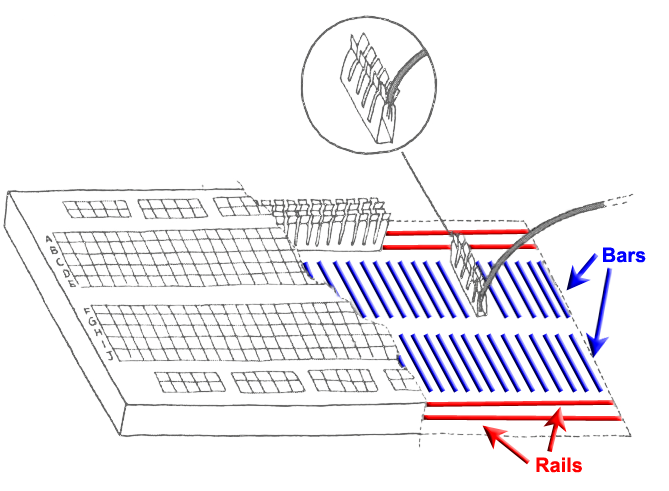
\includegraphics[width=0.9\textwidth]{microcontroller/breadboard-explosion.png}
        \caption{Breadboard connections}
    \end{figure}
\end{frame}

\begin{frame}{\glsentrydesc{led}}
    \begin{figure}
        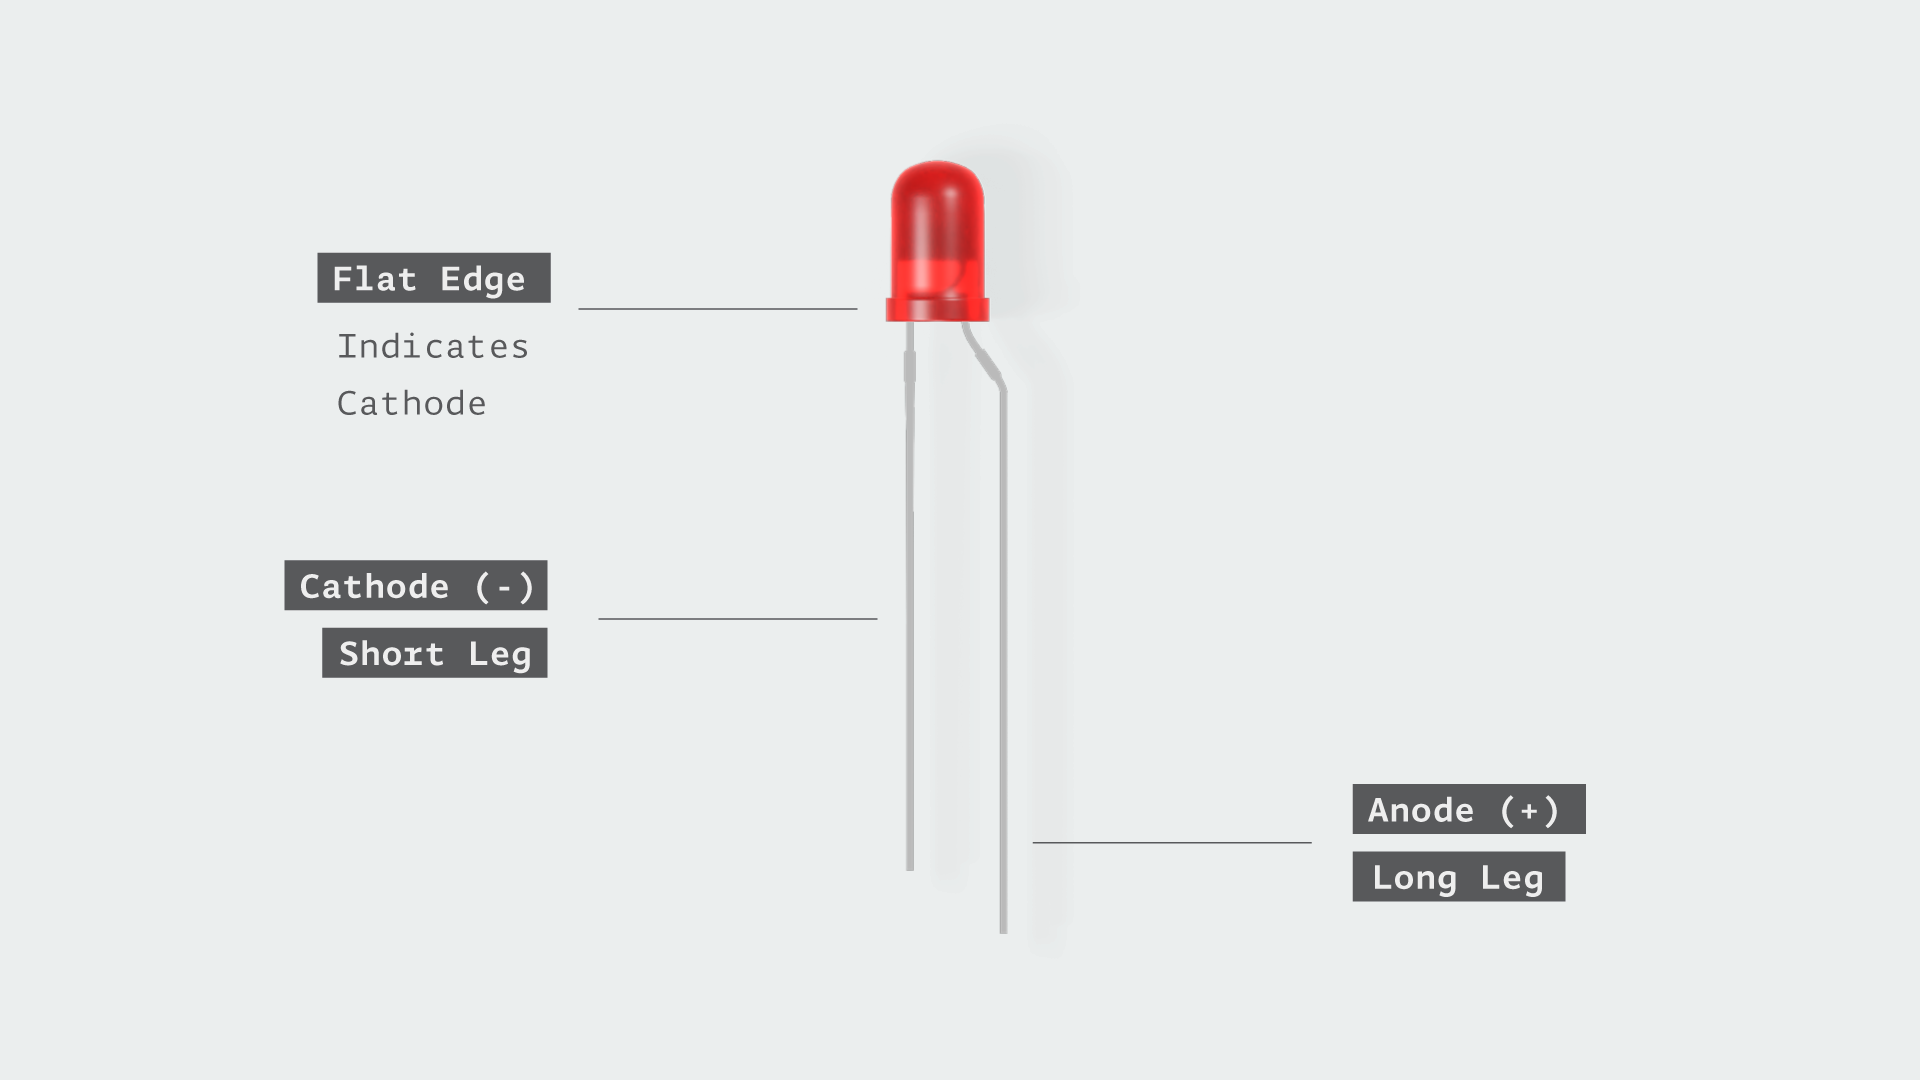
\includegraphics[width=0.9\textwidth]{microcontroller/leds.png}
        \caption{\glsentrytext{led} connections}
    \end{figure}
\end{frame}

\begin{frame}{Resistors}
    \begin{figure}
        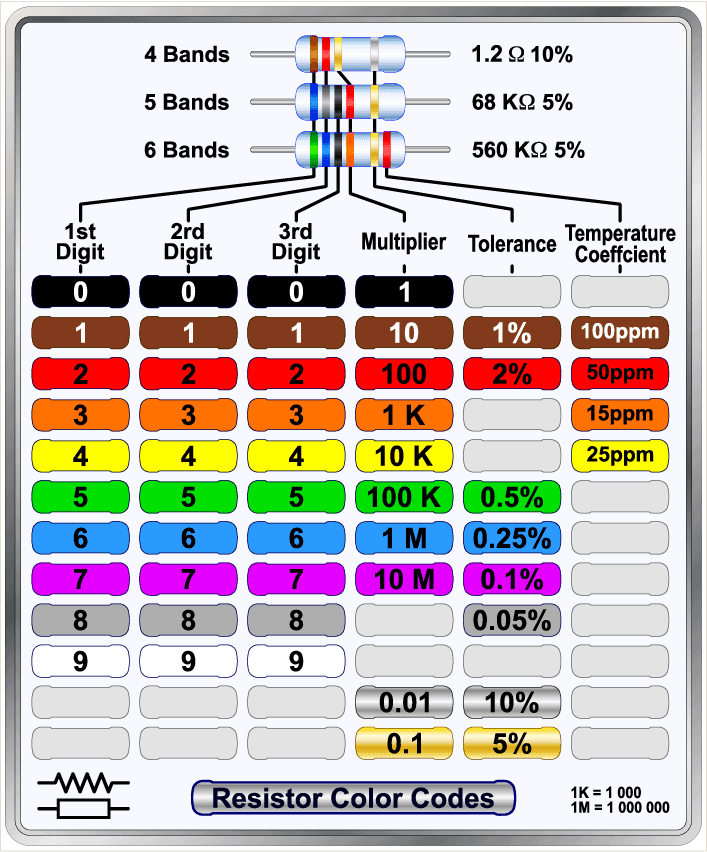
\includegraphics[width=0.55\textwidth]{microcontroller/resistor-color-code.png}
        \caption{Resistors color codes}
    \end{figure}
\end{frame}

\begin{frame}{Solution: Exercise II}
    \begin{listing}[H]
        \inputsource[fontsize=\fontsize{8}{8}]{c}{arduino/blink-external.c}
        \caption{Solution for Exercise II.}
        \label{lst:arduino:exercise:2:solution}
    \end{listing}
\end{frame}

\section{Exercise III: Blink MicroPython}

\begin{frame}
    \begin{exampleblock}{Exercise III}
        \begin{enumerate}
            \item Get the Arduino\textregistered{} \acs{ide} of your choice.
            \item Connect your board to your \acs{pc}.
            \item Install MicroPython on your board.
            \item Recreate the function of ``Exercise II''.
            \item Extend the example project to log \texttt{On} and \texttt{Off} to the console.% of your \acs{pc} when toggling the \acs{led}.
        \end{enumerate}
        % \par Hint:
        % \begin{itemize}
        %     \item \href{https://www.arduino.cc/reference/en/language/functions/communication/serial/begin/}{\mintinline{c}{Serial.begin()}}
        %     \item \href{https://www.arduino.cc/reference/en/language/functions/communication/serial/println/}{\mintinline{c}{Serial.println()}}
        % \end{itemize}
    \end{exampleblock}
\end{frame}

\begin{frame}{Solution: Exercise III}
    \begin{listing}[H]
        \inputsource[fontsize=\fontsize{8}{8}]{py}{arduino/blink-external.py}
        \caption{Solution for Exercise III.}
        \label{lst:arduino:exercise:3:solution}
    \end{listing}
\end{frame}

\section{Exercise IV: \glsentrytext{http} Request}

\begin{frame}
    \begin{exampleblock}{Exercise IV}
        \begin{enumerate}
            \item Connect your board to a network with internet connection.
            \item Perform a \acs{http} request to a website of your choice.
            \item Log the response of the web server to the terminal/console.
        \end{enumerate}
    \end{exampleblock}
\end{frame}

\begin{frame}{Solution: Exercise IV}
\end{frame}

\section{Exercise V: \glsentrytext{usb} Device}

\begin{frame}
    \begin{exampleblock}{Exercise V}
        \begin{enumerate}
            \item Connect your board to your \acs{pc}.
            \item Send control commands as \acs{usb} device.
        \end{enumerate}
    \end{exampleblock}
\end{frame}

\begin{frame}{Solution: Exercise V}
\end{frame}

\section{Exercise VI: \glsentrytext{iot} Cloud}

\begin{frame}
    \begin{exampleblock}{Exercise VI}
        \begin{enumerate}
            \item Create an Arduino\textregistered{} \acs{iot} Cloud project.
            \item Connect your \acs{rgb} \acs{led} to the \acs{iot} Cloud.
            \item Connect your \acs{imu} sensor values to the \acs{iot} Cloud.
        \end{enumerate}
    \end{exampleblock}
\end{frame}

\begin{frame}{Solution: Exercise VI}
\end{frame}

\section{Assignment: WebSocket}

\appendix

\begin{frame}[allowframebreaks]{Acronyms}
    \glsadd{ci}
    \glsadd{eth}
    \glsadd{gps}
    \glsadd{heidi}
    \glsadd{ir}
    \glsadd{lcd}
    \glsadd{mv}
    \glsadd{tft}
    \printglossary[type=\acronymtype, nonumberlist]
\end{frame}

% \begin{frame}[label=references]{References}
%     \bibliography{references}
% \end{frame}

\end{document}